% ch16a Electrons at strong coupling: Mottness, part a (书页 353-379 / 分册p001-027)
% 第16章 Electrons at strong coupling: Mottness
\chapter{强耦合电子：Mott性}

1986 年以前，对强相互作用电子系统的研究还是固体物理学中的一个边缘课题。铜氧化物陶瓷中高温超导电性的发现彻底改变了这种看法。原因很简单：未掺杂时，铜氧化物材料中含有一个部分填充的电子 $d$ 能带（[A1987]）。能带论告诉我们，部分填充的能带应当导电。然而，未掺杂的铜氧化物（cuprate）却是极好的绝缘体。尽管掺杂后它们变得导电，但它们表现出在大能量尺度上的谱权重重新分布，这是传统金属理论所无法理解的。能带论无法预言某些半填充能带中的绝缘态，正是莫特（Mott）在 1949 年（[M1949]）所处理的问题。莫特的分析源于他对 NiO 的研究：NiO 每个单胞含有两个未配对的 $d$ 电子，却依然是绝缘体。在大多数过渡金属氧化物中都能找到类似的绝缘态，最著名的是 $\mathrm{VO}_2$ 和 $\mathrm{V}_2\mathrm{O}_3$。由于能带论失效，莫特把目光聚焦到电子关联上，把它当作 NiO 绝缘态的根源。这一研究路线给出了固体物理学中一些最精妙的结果和最费解的问题。本章要讲述的，正是莫特态的物理，以及它在铜氧化物和其他体系中的种种表现。

固体物理学中的任何一个问题，一旦分离出了传播自由度，就可以认为已经被解决了。所谓传播自由度，是指那些使拉格朗日量成为二次型、并在单粒子格林函数中产生极点型奇异的激发。莫特问题之所以至今悬而未决，是因为存在一个内在困难：要把相互作用的拉格朗日量化成二次型，同时又不引入具有非正则对易关系的算符。在某种程度上，我们在第 12 章讲述费米液体理论时已经见过这类问题。然而，由于所有排斥性的短程相互作用都朝费米面重正化，它们的存在并不破坏费米液体底层自由粒子的图像。也就是说，可以把相互作用积掉，留下重正化的电子或准粒子态。因此，在费米液体中存在一条简单的原理，可以借此明白无疑地断定自由电子就是传播自由度。而没有费米面这一假设时，就不存在任何原理让我们把相互作用平滑掉。我们把这类问题称为强关联问题，即不存在像费米液体中那样的明显原理来支配电子--电子相互作用重正化的问题。在处理这种强耦合系统时，我们可以定义电荷流。然而，要赋予电荷流以粒子诠释，只有在传播自由度被确认之后才可能。强耦合下传播自由度的典型特征是：它们往往是复合激发，或是由基本构件构成的束缚态。著名的例子有量子色动力学——高能下的自由夸克在低能下形成束缚实体；还有硫化橡胶——其中一根根聚合物链失去各自的完整性，相互缠结成交联网络。分离这类集体现象是强耦合物理的核心问题。我们将证明，莫特问题也不例外。

\section{能带绝缘体}

为了理解莫特问题的特殊之处，让我们从能带绝缘体（band insulator）出发。我们把这样一个系统建模为电子在一条线性链上的跳跃，
\begin{equation*}
H_{\mathrm{BI}}=-t\sum_{j,\sigma}\left(c^{\dagger}_{j\sigma}c_{(j+1)\sigma}+c^{\dagger}_{(j+1)\sigma}c_{j\sigma}\right)+V\sum_{j,\sigma}(-1)^{j}c^{\dagger}_{j\sigma}c_{j\sigma}=H_{t}+H_{V},\tag{16.1}
\end{equation*}
链有 $N$ 个格点，并存在强度为 $V$ 的周期势（[S2010]）。虽然 $[H_{t},H_{V}]\neq 0$，但由于哈密顿量是二次的，两项仍可以同时对角化。作为跳跃项的结果，本征态是局域态的线性组合。因此，我们定义
\begin{equation*}
c_{n\sigma}=\frac{1}{\sqrt{N}}\sum_{k\sigma}\mathrm{e}^{\mathrm{i}kna}c_{k\sigma}\tag{16.2}
\end{equation*}
借助于傅里叶振幅 $c_{k\sigma}$。把式 (16.2) 代入跳跃项，
\begin{equation*}
H_{t}=-\frac{t}{N}\sum_{n,k,k',\sigma}\left(\mathrm{e}^{-\mathrm{i}kna}\mathrm{e}^{\mathrm{i}k'(n+1)a}c^{\dagger}_{k\sigma}c_{k'\sigma}+\mathrm{e}^{\mathrm{i}kna}\mathrm{e}^{-\mathrm{i}k'(n+1)a}c^{\dagger}_{k'\sigma}c_{k\sigma}\right),\tag{16.3}
\end{equation*}
再结合
\begin{equation*}
\frac{1}{N}\sum_{n}\mathrm{e}^{\mathrm{i}kna}\mathrm{e}^{-\mathrm{i}k'na}=\delta_{k-k'},\tag{16.4}
\end{equation*}
便得到
\begin{equation*}
H_{t}=\sum_{k\sigma}\epsilon(k)c^{\dagger}_{k\sigma}c_{k\sigma}={\sum_{k\sigma}}'\epsilon(k)c^{\dagger}_{k\sigma}c_{k\sigma}-\epsilon(k)c^{\dagger}_{(k-\pi/a)\sigma}c_{(k-\pi/a)\sigma},\tag{16.5}
\end{equation*}
其中 $\epsilon(k)=-2t\cos ka$，求和号上的撇号表示把 $k$ 限制在 $[-\pi/2a,\pi/2a]$ 内。类似地，周期势项变为
\begin{equation*}
H_{V}=\frac{V}{N}\sum_{n,k,k'\sigma}\mathrm{e}^{\mathrm{i}n(ka-k'a+\pi)}c^{\dagger}_{k'\sigma}c_{k\sigma}={\sum_{k\sigma}}'\left(c^{\dagger}_{k\sigma}c_{(k-\pi/a)\sigma}+\mathrm{h.c.}\right).\tag{16.6}
\end{equation*}
对称化跳跃项之后，我们写出完整哈密顿量
\begin{equation*}
H_{\mathrm{BI}}=H_{t}+H_{V}={\sum_{k\sigma}}'\Psi^{\dagger}_{k\sigma}\begin{pmatrix}\epsilon(k) & V\\ V & -\epsilon(k)\end{pmatrix}\Psi_{k\sigma}\tag{16.7}
\end{equation*}

\begin{figure}[H]\centering
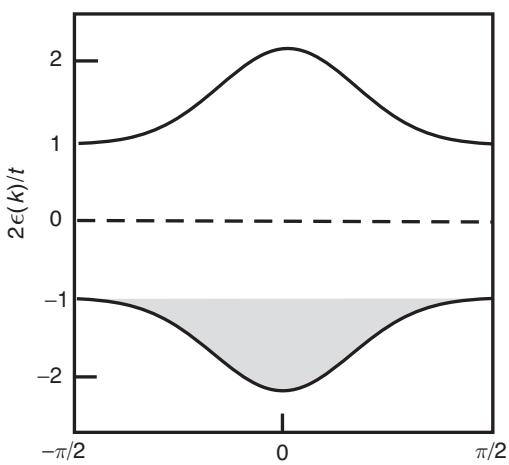
\includegraphics[width=0.55\textwidth]{figs/ch16/fig_16.1.jpg}
\caption*{图 16.1\quad 能带绝缘体的能带结构，以跳跃积分 $t$ 为单位，周期势强度为 $V=t$。价带（阴影区）是满的，而上面的带（导带）是空的。}\label{fig:auto:16.1}
\end{figure}

并以矩阵形式写为
\begin{equation*}
\Psi_{\sigma}=\begin{pmatrix}c_{k\sigma}\\ c_{(k-\pi/a)\sigma}\end{pmatrix}.\tag{16.8}
\end{equation*}
这个哈密顿量矩阵可以立即对角化。其本征值为
\begin{equation*}
\varepsilon(k)=\pm\sqrt{V^{2}+\epsilon(k)^{2}}.\tag{16.9}
\end{equation*}
于是出现了两条能带，如图 16.1 所示：下面带阴影的一条是填满的价带，上面一条是空的导带，它们分别对应于 $c_{k\sigma}$ 与 $c_{(k-\pi/a)\sigma}$ 的成键与反键组合。只要价带是满的，往系统中再放入一个额外的电子就要付出等于 $2V$ 的能隙。

于是，价带和导带在非相互作用哈密顿量的正交本征态语言中有简单的诠释。当然，任何材料中的电子都相互作用。那么，在存在相互作用时，导带和价带是否还有相应简单的诠释？这是一个微妙的问题。如果存在一个保护能隙的不动点，回答起来最容易。而确立这样一个不动点，需要对我们的晶格模型取连续极限。这种极限的困难立刻显现。用晶格常数表示，晶格的长度为
\begin{equation*}
L=Na.\tag{16.10}
\end{equation*}
连续极限对应于 $N\to\infty$ 且 $a\to 0$，同时 $L$ 保持固定。微妙之处出在粒子数上。如果保持粒子数固定，那么粒子填充数 $N_{\mathrm{p}}/N$ 在连续极限下实际上趋于零。也就是说，晶格模型的连续极限严格来说只在低密度极限下才有效，此时只有带底或者说低动量的态被占据。通过把式 (16.2) 改写为
\begin{equation*}
\frac{c_{n\sigma}}{\sqrt{a}}=\frac{1}{\sqrt{L}}\sum_{k\sigma}\mathrm{e}^{\mathrm{i}kx}c_{k\sigma},\tag{16.11}
\end{equation*}
即显式地以其对 $L$ 的依赖来表达（其中 $x=na$），我们可以形式化地得出同样的结论。由这个表达式可以清楚地看到，右端只依赖于 $x$，因为它对所有 $k$ 求和。因此，左端也必须只依赖连续变量 $x$。于是我们建立如下对应
\begin{equation*}
\psi_{\sigma}(x)=\lim_{a\to 0}\left.\frac{c_{n\sigma}}{\sqrt{a}}\right|_{x}\tag{16.12}
\end{equation*}
即在连续场 $\psi_{\sigma}(x)$（它在 $x$ 处湮灭一个粒子）与其晶格对应物之间。式 (16.11) 只有在右端存在有限个产生算符时才有意义，否则结果是无穷大。也就是说，连续极限对应于在无穷多个格点上产生有限个粒子。因此，密度必定为零。带底的态具有比晶格常数大得多的波长。而带顶的态——正是与描述能隙相关的那些态——具有大动量。因此，连续极限对解决这个问题毫无用处。当然，一个例外是能隙打开在狄拉克点处的情形，这时关于带底的连续极限才是相关的。

真正把能带绝缘体问题与莫特绝缘体区分开的，是前者的能带是刚性的而后者的不是。在没有相互作用时，能带绝缘体由严格作为单粒子（或单电子）算符本征态的能带构成。因此，改变价带中的粒子数对导带毫无影响，如图 16.2 所示。在未掺杂系统中，每条能带每格点的态的总数为 2（图 16.2）。任何态密度按图 16.2 方式演化的系统都与能带绝缘体等价，例如半导体。正如我们将看到的，在莫特问题中，即使在该能隙可以不依赖维度精确求解的极限下，出现的能带也不是刚性的。在掺杂莫特绝缘体的任何极限下，都不存在类似图 16.2 的图像。事实上，甚至每条能带携带的总谱权重也依赖于电子填充数。也就是说，“高能带”的含义依赖于较低能带中的占据情况。其结果是，莫特能隙没有单电子诠释。事实上，根本不可能用具有正则对易关系的粒子来诠释它。因此，莫特问题从根本上是关于复合对象的问题。既然莫特能带的非刚性是莫特问题的内在特征，我们引入了 Mott 性（Mottness）这个术语，用以指称与这种非刚性相伴的所有实验上可观测的性质。

\begin{figure}[H]\centering
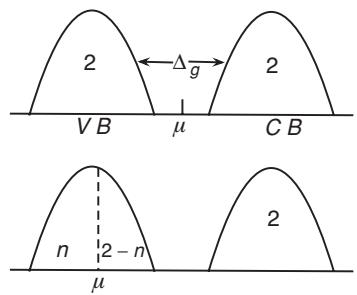
\includegraphics[width=0.55\textwidth]{figs/ch16/fig_16.2.jpg}
\caption*{图 16.2\quad 能带绝缘体中单粒子态密度随电子填充数 $n$ 的演化。VB 与 CB 分别对应价带与导带。价带的总权重是常数 2，即每格点 2 个态。掺杂只是把一个态推到化学势之上。化学势以下态密度的积分总是等于填充数 $n$。}\label{fig:auto:16.2}
\end{figure}

\section{莫特问题}

莫特 1949 年的论文（[M1949]）由两部分组成。在第一部分，他完全基于势能的考虑，对 NiO 的绝缘态给出了一个简单的解释。在论文的后半部分，他详尽地讨论了为什么这个简单的图像实际上行不通。简言之，它忽略了量子力学！此后文献中似乎随之出现了一种不幸的遗忘症：简洁性压倒了准确性。

NiO 的一个单胞含有偶数个未配对电子，却仍然绝缘。为看清这一点，考虑 NiO 的轨道组态。Ni 是 $4s^{2}3d^{8}$，O 是 $2s^{2}2p^{4}$。Ni 的两个 $4s$ 电子被交给氧，从而填满 $2p$ 壳层，使 Ni 处于 $+2$ 价态。于是，NiO 中外壳层的 $d$ 壳层有两个未配对电子。因此，按能带图像它被预期会导电。然而它具有电荷能隙。为解释这个能隙，莫特求助于电子之间的相互作用。在莫特的构造中，对窄 $d$ 能带占主导的相关相互作用是把两个电子放到同一个 Ni 原子上所需的能量代价
\begin{equation*}
U=E^{N+1}+E^{N-1}-2E^{N},\tag{16.13}
\end{equation*}
其中 $E^{N}$ 是具有 $N$ 个价电子的原子的基态能量。除去填满的壳层，Ni 的 $N=2$。莫特推断，在零温下，如果 $U$ 超过一个临界值（典型地为能带宽度的量级），就不存在具有 $N\pm 1$ 个电子的 Ni 原子。也就是说，所有 Ni 原子都是 $+2$ 价，因而不发生导电，如图 16.3 所示。按照这一论证，由此产生的电荷能隙就是用自旋向上和自旋向下的电子双重占据同一格点所需的能量代价。于是，这个简单的哈密顿量
\begin{equation*}
H_{\mathrm{Hubb}}=-t\sum_{i,j,\sigma}g_{ij}c^{\dagger}_{i\sigma}c_{j\sigma}+U\sum n_{i\uparrow}n_{i\downarrow}-\mu\sum_{i,\sigma}n_{i\sigma},\tag{16.14}
\end{equation*}

\begin{figure}[H]\centering
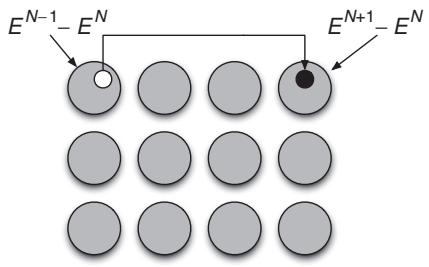
\includegraphics[width=0.62\textwidth]{figs/ch16/fig_16.3.jpg}
\caption*{图 16.3\quad 莫特所设想的半填充能带。每个圆圈代表一个具有 $N$ 个电子、基态能量为 $E^{N}$ 的中性原子。图中明确标出了移走电子与加入电子的能量差。莫特推断不存在双占据格点，因为在零温下 $U=E^{N+1}+E^{N-1}-2E^{N}\gg 0$。当然，这并不成立。因此，必须把莫特能隙理解为动力学的而非静态的。}\label{fig:auto:16.3}
\end{figure}

最早由哈伯德（Hubbard）引入（[H1963]）：电子在一组格点之间以矩阵元 $t$ 跳跃，但每当它们双重占据同一格点时就要付出能量代价 $U$。这个模型足以描述向莫特所设想的态的转变。在这个模型中，$i,j$ 标记格点，当且仅当 $i,j$ 为最近邻时 $g_{ij}$ 等于 1，$c_{i\sigma}$ 湮灭格点 $i$ 上自旋为 $\sigma$ 的一个电子，$t$ 是最近邻跳跃矩阵元。由式 (16.14) 可见，基态中既不存在 $\mathrm{Ni}^{+++}$ 也不存在 $\mathrm{Ni}^{+}$ 离子这一简单的莫特图像，只在跳跃为零时才成立。这就是原子极限，也就是莫特论文第一部分给出的论证。

我们可以把莫特的第一个论证表述得更精确。哈伯德模型由两个不对易的项组成。与 $H_{\mathrm{BI}}$ 不同，哈伯德模型在电子算符上不是二次的，因此势能项与动能项的不对易性构成了一个实质性的困难。尽管如此，通过把电子湮灭算符写成
\begin{equation*}
c_{i\sigma}=c_{i\sigma}(1-n_{i\bar{\sigma}})+c_{i\sigma}n_{i\bar{\sigma}}=\xi_{i\sigma}+\eta_{i\sigma},\tag{16.15}
\end{equation*}
即两个算符之和（其中每一个都只作用于某一类格点），哈伯德模型仍可以被化成二次型。算符 $\xi_{i\sigma}$ 从单占据的格点上湮灭一个电子，而 $\eta_{i\sigma}$ 从双占据的格点上湮灭一个电子。注意到对费米子有 $n^{2}_{i\sigma}=1$，可得 $n_{i\uparrow}n_{i\downarrow}=n_{i\uparrow}n^{2}_{i\downarrow}=\eta^{\dagger}_{i\uparrow}\eta_{i\uparrow}$，这表明相互作用项
\begin{equation*}
H_{U}=U\sum_{i}n_{i\uparrow}n_{i\downarrow}=\frac{U}{2}\sum_{i\sigma}\eta^{\dagger}_{i\sigma}\eta_{i\sigma},\tag{16.16}
\end{equation*}
可以完全用 $\eta_{i\sigma}$ 写成二次型。对动能项也可以如法炮制：只需代入式 (16.15)，即可把哈伯德模型
\begin{equation*}
H_{\mathrm{Hubb}}=-t\sum_{i,j,\sigma}\left(\eta^{\dagger}_{i\sigma}\eta_{j\sigma}+\xi^{\dagger}_{i\sigma}\xi_{j\sigma}+\eta^{\dagger}_{i\sigma}\xi_{j\sigma}+\xi^{\dagger}_{j\sigma}\eta_{i\sigma}\right)+\frac{U}{2}\sum_{i,\sigma}\eta^{\dagger}_{i\sigma}\eta_{i,\sigma},\tag{16.17}
\end{equation*}
完全改写成二次型。事实证明，这种类型的变换在任何相互作用问题中总能做到。复杂之处在于，$\xi_{i\sigma}$ 与 $\eta_{j\sigma}$ 算符服从非正则的对易关系
\begin{align*}
\{\eta_{i\alpha},\xi_{j\beta}\}=\delta_{ij}c_{i\beta}c_{j\alpha},\\
\{\eta_{i\alpha},\eta^{\dagger}_{j\beta}\}=\delta_{ij}(n_{i\bar{\alpha}}\delta_{\alpha\beta}-c^{\dagger}_{i\beta}c_{i\alpha}\delta_{\bar{\alpha}\beta}),\\
\{\xi_{i\alpha},\xi^{\dagger}_{j\beta}\}=\delta_{ij}((1-n_{i\bar{\alpha}})\delta_{\alpha\beta}+c^{\dagger}_{i\beta}c_{i\alpha}\delta_{\bar{\alpha}\beta}),\\
\{\eta_{i\alpha},\eta_{j\beta}\}=\{\xi_{i\alpha},\xi_{j\beta}\}=\{\xi_{i\alpha},\eta^{\dagger}_{j\beta}\}=0.\tag{16.18}
\end{align*}
虽然相互作用项在这个新基下是对角的，跳跃项却不是。它显式地混合双占据与单占据两个分部。因此，$\eta_{i\sigma}$ 与 $\xi_{i\sigma}$ 算符构成了哈伯德模型强耦合展开的基。既然这些算符把相互作用对角化，把它们当作单粒子福克（Fock）空间中的对象来思考是错误的。也就是说，在这个新基下，威克（Wick）定理根本无从定义。

考虑原子极限。由于所有本征态都是局域粒子占据数的本征态，它们可以按所含双占据格点的数目排序。在半填充时，基态每格点有一个电子。第一激发态有一个双占据，依此类推。到第一激发态的能隙恰好是 $U$。这就是莫特的图像：基态中每个原子都是中性的，能隙代表到第一个含双占据的态的能量差。

无论 $t=0$ 的图像多么初始，它仍以最简单的形式包含了 Mott 性。也就是说，由 $\eta_{i\sigma}$ 与 $\xi_{i\sigma}$ 产生的能带不是静止的：它们携带的总谱权重依赖于填充数。换言之，由 $\eta_{i\sigma}$ 与 $\xi_{i\sigma}$ 定义的不是传统能带绝缘体图像中的能带。我们将用两种方式来说明这一点。首先，正如格林函数一节中的式 (7.100) 所示，一条能带的总谱强度由在该能带中产生粒子的算符的反对易关系给出。下能带（$\xi_{i\sigma}$ 带）中的谱权重完全由
\begin{equation*}
m^{0}_{\mathrm{LHB}}=\frac{1}{N}\sum_{i,\sigma}\langle\{\xi_{i\sigma},\xi^{\dagger}_{i\sigma}\}\rangle=2-n=1+x,\tag{16.19}
\end{equation*}
给出，其中我们用到了式 (16.18)，$x$ 是引入下能带的空穴数目。空穴数是相对半填充定义的，因而 $n\equiv\langle(n_{i\downarrow}+n_{i\uparrow})\rangle=1-x$。由于上、下两条带之间的总权重必须是 2，上能带中的权重必定是
\begin{equation*}
m^{0}_{\mathrm{UHB}}=\frac{1}{N}\sum_{i,\sigma}\langle\{\eta_{i\sigma},\eta^{\dagger}_{i\sigma}\}\rangle=n=1-x\tag{16.20}
\end{equation*}
（原子极限下）。如果我们关心的是电子掺杂，这些权重就会对调。第一个显而易见的事实是：在半填充 $x=0$ 处，下能带与上能带

\begin{figure}[H]\centering
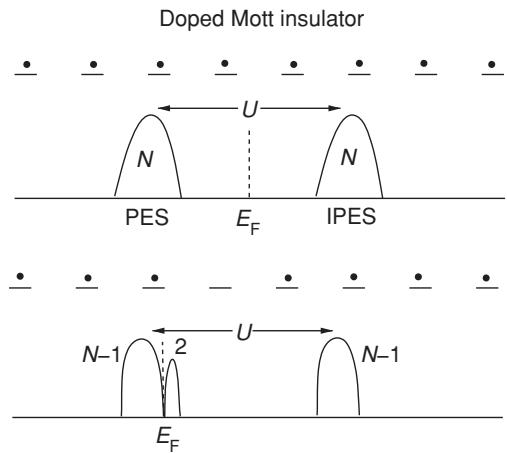
\includegraphics[width=0.60\textwidth]{figs/ch16/fig_16.4.jpg}
\caption*{图 16.4\quad (a) 大 $U\gg t$ 极限下的半填充能带在单粒子谱中产生能隙。图中所示的带代表上、下哈伯德带（upper/lower Hubbard band）。在 $N$ 格点系统中，半填充时每条带中的单粒子态总数为 $N$。电子移走即光电子发射（PES）带与电子加入即反光电子发射（IPES）带，分别对应于电子在空格点上与在单占据格点上运动。原子极限下两带的劈裂为 $U$。(b) 哈伯德模型原子极限下，掺杂莫特绝缘体从半填充到单空穴极限的单粒子态密度演化。移走一个电子会在低能处产生两个空态，而能带绝缘体极限下只有一个。与费米液体的关键差别在于：下哈伯德带（对应费米液体中的价带）携带的总谱权重不是常数，而是填充数的函数。}\label{fig:auto:16.4}
\end{figure}

携带相同的谱权重。与之形成鲜明对照的是能带绝缘体：在绝缘态中只有价带具有谱权重。此外，在任何有限掺杂下，谱权重都依赖于掺杂水平，这也与能带绝缘体中它严格为常数形成对照。这一差别完全源于：即使在 $t=0$ 时，莫特问题中的能隙也不是用单电子算符定义的。也就是说，与式 (16.1) 不同，任何极限下莫特能隙背后都没有单电子图像。尽管如此，原子极限中上、下能带谱权重的掺杂依赖背后有一个简单的物理图像。考虑图 16.4。在原子极限的半填充下，在 $N$ 格点系统中恰好有 $N$ 种方式加入或移走一个电子。因此，光电子发射带与反光电子发射带各有 $N$ 个态。在能带绝缘体中，一个空穴在价带中产生单个空态，而导带不受影响。莫特绝缘体即使在半填充时也不是这样。考虑产生一个空穴。现在有 $N-1$ 种方式移走一个电子，同样也有 $N-1$ 种方式产生双占据。然而我们必须保持态数守恒。这两个尚未得到解释的神秘态，对应于用自旋向上或自旋向下电子去占据那个空格点的两种方式。因此，每个空格点的总谱权重是 2。由于把电子放进这两个态中的任何一个都不耗能量，这些态必定恰好位于化学势之上，构成下能带的空的部分，如图 16.4 所描绘。当引入 $n_{\mathrm{h}}$ 个空穴使得 $x=n_{\mathrm{h}}/N$ 时，下能带中的总权重为 $1+x$。化学势以下的权重为 $1-x$，而化学势以上有 $2x$ 个态。注意，化学势以下的权重与上能带中的权重完全相同，因为上能带中的权重只有当格点已经被单占据时才存在。因此，在原子极限下，上、下能带中化学势以下的权重必定互为镜像。这种镜像关系在偏离原子极限后以何种方式延续，是莫特问题真正的微妙之处之一。

\subsection{格林函数：原子极限}

证明哈伯德模型中每条能带的权重依赖于填充数的第二种方式，是直接计算单粒子格林函数。遵循第 7 章，我们把相关的推迟格林函数定义为
\begin{equation*}
G^{\mathrm{R}}_{i\sigma}(t,0)=-\mathrm{i}\theta(t)\langle\{c_{i\sigma}(t),c^{\dagger}_{i\sigma}(0)\}\rangle,\tag{16.21}
\end{equation*}
它在格点空间中是纯对角的。一般情形并非如此，正如我们在对完整哈伯德模型的更完整处理中将会看到的。在原子极限下，利用运动方程技巧可以把格林函数推导成闭合形式。对两边求导，得到
\begin{equation*}
\partial_{t}G^{\mathrm{R}}_{i\sigma}(t,0)=-\mathrm{i}\delta(t)-\mathrm{i}\theta(t)\langle\{\dot{c}_{i\sigma},c^{\dagger}_{i\sigma}\}\rangle,\tag{16.22}
\end{equation*}
其中第一项来自对亥维赛（Heaviside）阶跃函数求导。由海森堡运动方程
\begin{equation*}
\mathrm{i}\dot{c}_{i\sigma}=\frac{U}{\hbar}c_{i\sigma}n_{i\bar{\sigma}}-\frac{\mu}{\hbar}c_{i\sigma},\tag{16.23}
\end{equation*}
出发，再引入一个附加的格林函数是明智的，
\begin{equation*}
\tilde{G}^{\mathrm{R}}_{i\sigma}(t,0)=-\mathrm{i}\theta(t)\langle\{c_{i\sigma}(t)n_{i\bar{\sigma}}(t),c^{\dagger}_{i\sigma}(0)\}\rangle.\tag{16.24}
\end{equation*}
把式 (16.23) 代入式 (16.22)，
\begin{equation*}
\partial_{t}G^{\mathrm{R}}_{i\sigma}(t,0)=-\mathrm{i}\delta(t)-\mathrm{i}\frac{U}{\hbar}\tilde{G}^{\mathrm{R}}_{i\sigma}(t,0)+\mathrm{i}\frac{\mu}{\hbar}G^{\mathrm{R}}_{i\sigma}(t,0),\tag{16.25}
\end{equation*}
暴露出运动方程方法的内在困难，即对一系列其他格林函数的层层嵌套依赖。幸运的是，在原子极限下方程可以封闭，因为 $\tilde{G}^{\mathrm{R}}_{i\sigma}(t,0)$ 的导数
\begin{equation*}
\partial_{t}\tilde{G}^{\mathrm{R}}_{i\sigma}(t,0)=-\mathrm{i}\delta(t)\langle\{c_{i\sigma}n_{i\bar{\sigma}},c^{\dagger}_{i\sigma}\}\rangle-\mathrm{i}\theta(t)\langle\{\dot{c}_{i\sigma}(t)n_{i\bar{\sigma}}(t),c^{\dagger}_{i\sigma}\}\rangle,\tag{16.26}
\end{equation*}
约化成一个简单的函数，
\begin{equation*}
\partial_{t}\tilde{G}^{\mathrm{R}}_{i\sigma}(t,0)=-\mathrm{i}\delta(t)\langle n_{i\bar{\sigma}}\rangle-\mathrm{i}\frac{U}{\hbar}\tilde{G}^{\mathrm{R}}_{i\sigma}(t,0)+\mathrm{i}\frac{\mu}{\hbar}\tilde{G}^{\mathrm{R}}_{i\sigma}(t,0).\tag{16.27}
\end{equation*}
在简化这个方程时，我们用到了运动方程即式 (16.23)，以及 $\dot{n}_{i\sigma}=0$ 和 $n^{2}_{i\sigma}=n_{i\sigma}$ 这两个事实。余下的现在很简单。引入傅里叶变换
\begin{equation*}
f(\omega)=\int_{-\infty}^{\infty}\mathrm{e}^{\mathrm{i}\omega t/\hbar}f(t)\mathrm{d}t,\tag{16.28}
\end{equation*}
我们发现
\begin{equation*}
\tilde{G}^{\mathrm{R}}_{i\sigma}(\omega)=\frac{\hbar n_{i\bar{\sigma}}}{\omega-U+\mu}\tag{16.29}
\end{equation*}
从而
\begin{equation*}
G^{\mathrm{R}}_{i\sigma}(\omega)=\hbar\left(\frac{1}{\omega+\mu}+\frac{U\langle n_{i\bar{\sigma}}\rangle}{(\omega+\mu)(\omega+\mu-U)}\right),\tag{16.30}
\end{equation*}
其中已默认 $\omega$ 具有正的虚部。如果把方程按部分分式分解，其物理含义会更加直白：
\begin{equation*}
G^{\mathrm{R}}_{i}(\omega)=\frac{1}{\hbar}\sum_{\sigma}G^{\mathrm{R}}_{i\sigma}(\omega)=\frac{2-n}{\omega+\mu}+\frac{n}{\omega+\mu-U},\tag{16.31}
\end{equation*}
这揭示出潜在的双极点结构。通过作平移 $\mu\to\mu+\frac{U}{2}$ 并对空穴掺杂系统取 $n=1-x$，我们得到一个更对称的表达式
\begin{equation*}
G^{\mathrm{R}}_{i}(\omega)=\frac{1+x}{\omega+\mu+\frac{U}{2}}+\frac{1-x}{\omega+\mu-\frac{U}{2}},\tag{16.32}
\end{equation*}
两个极点相距 $U$，分别携带谱权重 $1+x$ 与 $1-x$。每个空穴从高能部分移走一个单态，从而给出 $1-x$ 的留数。这个空态在低能处重新出现，成为低能加入谱的一部分。谱的空的部分按 $2x$ 而非能带绝缘体中的 $x$ 增长，这一事实正体现了这种静态的谱权重转移。这里“静态”一词的意思是：谱权重可以仅凭电子态计数来解释。正如我们将看到的，还存在一种附加的动力学效应，它无法用这种态计数来枚举。读者应当记住，在莫特体系中用“能带”一词指称化学势上下谱权重开始出现的位置，与能带绝缘体标准的刚性带图像相比，携带着一套根本不同的观念，尤其是谱权重转移。

在思考原子极限时，引入霍尔丹（Haldane）对泡利原理的推广（[H1991]）是有帮助的。霍尔丹指出，我们可以把统计
\begin{equation*}
\Delta d_{\alpha}=-\sum_{\beta}g_{\alpha\beta}\Delta N_{\beta},\tag{16.33}
\end{equation*}
完全理解为：当类型 $\beta$ 的粒子数增加 $\Delta N_{\beta}$ 时，加入类型 $\alpha$ 粒子的可用态数如何变化（$\Delta d_{\alpha}$）。这里 $g_{\alpha\beta}$ 是统计矩阵，它决定类型 $\alpha$ 与 $\beta$ 粒子的希尔伯特空间如何相互影响。考虑自旋向上或向下的简单情形。对无相互作用电子，$g_{\alpha\beta}=\delta_{\alpha\beta}$。也就是说，加入自旋向上电子的相空间与自旋向下电子的数目无关。在哈伯德模型的 $U=\infty$ 原子极限下，每格点只能有一个电子。因此，自旋向上与自旋向下电子的希尔伯特空间是相互关联的，$g$ 矩阵为
\begin{equation*}
g=\begin{pmatrix}1 & 1\\ 1 & 1\end{pmatrix},\tag{16.34}
\end{equation*}

\begin{figure}[H]\centering
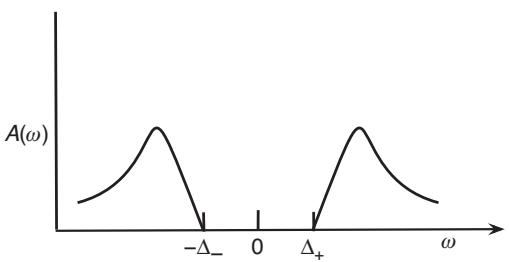
\includegraphics[width=0.60\textwidth]{figs/ch16/fig_16.5.jpg}
\caption*{图 16.5\quad 半填充系统中的谱函数随频率的变化。$\pm\Delta_{\pm}$ 表示莫特能隙的下（$-$ 号）与上（$+$ 号）边缘。}\label{fig:auto:16.5}
\end{figure}

具有非对角元。由于每个粒子都排斥其他粒子占据同一格点，服从式 (16.34) 的粒子有时被称为排除子（excluson）。式 (16.34) 清楚表明：电子之间的相互作用在某些情况下可以被改写成一条新的统计原理。偏离 $U=\infty$ 极限时，这一点不再成立。

\section{大做文章的零点：卢廷格表面}

能带绝缘体与莫特绝缘体之间还有另一个差别，可以用哈伯德模型的原子极限来说明。为说明这一点，我们计算原子极限下的谱函数
\begin{align*}
A(\omega)&=-\frac{1}{\pi}\mathrm{Im}\,G^{\mathrm{R}}_{i}(\omega+\mathrm{i}\Gamma)\\
&=\left((1+x)\delta(\omega-\mu+U/2)+(1-x)\delta(\omega-\mu-U/2)\right),\tag{16.35}
\end{align*}
在能带绝缘体中，化学势之上的那条带没有任何谱权重。莫特绝缘体则不然。这带来一个深远的后果。由克拉默斯--克勒尼希（Kramers--Kronig）关系，推迟格林函数的实部
\begin{equation*}
R(\omega)\equiv\mathrm{Re}\,G^{\mathrm{R}}_{i}(\omega)=\int_{-\infty}^{\infty}\mathrm{d}\omega'\frac{A(\omega')}{\omega-\omega'},\tag{16.36}
\end{equation*}
与谱函数直接相关。我们关心的是这个积分在半填充系统中零频处的行为。由于谱函数在莫特能隙内为零，这个积分在零频（即粒子--空穴对称情形下化学势所在的位置）简化为
\begin{equation*}
R(0)=-\int_{-\infty}^{-\Delta_{-}}\frac{A(\omega')}{\omega'}\mathrm{d}\omega'-\int_{\Delta_{+}}^{\infty}\frac{A(\omega')}{\omega'}\mathrm{d}\omega',\tag{16.37}
\end{equation*}
其中 $\Delta_{-}$ 与 $\Delta_{+}$ 是莫特能隙的下、上边缘，如图 16.5 所描绘。对能带绝缘体而言，这个积分没有什么特殊意义。然而在莫特体系中，即使超出原子极限，这个积分也有可能（[D2003]）为零，原因很简单：谱函数在化学势上下总是正的且非零。第一项的积分为负，第二项为正。因此 $R(0)$ 可以为零。在 $x=0$ 的原子极限下，这个计算可以显式完成：
\begin{equation*}
R(0)=-\int_{-\infty}^{-\Delta_{-}}\frac{\delta(\omega'-\mu+U/2)}{\omega'}\mathrm{d}\omega'-\int_{\Delta_{+}}^{\infty}\frac{\delta(\omega'-\mu-U/2)}{\omega'}\mathrm{d}\omega',\tag{16.38}
\end{equation*}
它在 $\mu=0$ 时对所有动量都为零。$R(0)$ 对所有动量为零这一条件只在原子极限下成立。偏离该极限时，由于谱函数具有显式的动量依赖，零点条件将依赖于动量。莫特绝缘体的严格定义是：\emph{任何部分填充的能带，只要在顺磁态下相应的推迟格林函数在化学势的某个取值处沿动量空间中一个连通曲面实部为零}。这样的曲面定义了所谓的卢廷格表面（Luttinger surface），它的出现完全是因为莫特绝缘体在化学势上下都有非零的谱函数。能带绝缘体不存在这样的曲面。莫特绝缘体中零点面的意义在于：电子传播子正是沿着这个曲面消失。不出所料，电子并不是传播自由度。“零点面只对化学势的某个取值存在”这一限制条件是本质性的，因为从式 (16.38) 可以清楚看到，只有在粒子--空穴对称点上才有 $R(0)=0$。在不可压缩态中，化学势的放置带有任意性（[R2007]），因为能隙内的任何位置都能保持莫特态的绝缘性质。

偏离原子极限时，我们仍可以确立（[SPC2007]）零点面的确切位置，而无需显式计算谱函数——但前提是哈密顿量具有粒子--空穴对称性。由式 (16.37)，我们只需确定谱函数对频率为偶函数的那些动量。为此，考虑一个一般的粒子--空穴变换
\begin{equation*}
c_{i\sigma}\to\mathrm{e}^{\mathrm{i}\mathbf{Q}\cdot\mathbf{r}_{i}}c^{\dagger}_{i\sigma},\tag{16.39}
\end{equation*}
作用于电子湮灭算符。哈密顿量在该变换下保持不变，这同时对 $\mathbf{Q}$ 和化学势提出了约束。具有最近邻跳跃的哈伯德模型在 $\mathbf{Q}=(\pi,\pi)$、$\mu=U/2$ 下在式 (16.39) 变换下保持不变。后者正是半填充即莫特态下的化学势取值。回想在推导式 (16.32) 时，我们通过变换 $\mu\to\mu+U/2$ 关于 $U/2$ 作了对称化。把格林函数
\begin{equation*}
G^{\mathrm{R}}_{ij\sigma}(t,0)=-\mathrm{i}\theta(t)\langle\{c_{i\sigma}(t),c^{\dagger}_{j\sigma}(0)\}\rangle,\tag{16.40}
\end{equation*}
中的算符按式 (16.39) 变换，利用式 (7.95) 与式 (7.97)，并把化学势固定在 $\mu=U/2$，便得到恒等式
\begin{equation*}
A_{\sigma}(\omega,\mathbf{k})=A_{\sigma}(-\omega,-\mathbf{k}-\mathbf{Q}+2n\pi).\tag{16.41}
\end{equation*}
因此，对 $\mathbf{k}=\mathbf{Q}/2+n\pi$，谱函数是频率的偶函数。在这些动量上，式 (16.37) 中的积分为零。考虑一维并取最近邻跳跃。此时对称点是 $\pm\pi/2$，即半填充无相互作用能带的费米点。在二维中，这个证明只足以确立两个点，而非一个零点面。为确定曲面，我们利用高维中的一种附加对称性。例如在二维中，只有当跳跃各向同性时，我们才能交换正则 $(x,y)$ 轴而保持哈密顿量不变。这种不变性允许我们在式 (16.41) 的左端交换 $k_{x}$ 与 $k_{y}$，得到条件
\begin{equation*}
k_{y}=-k_{x}-q+2n\pi\tag{16.42}
\end{equation*}
再由反射对称性
\begin{equation*}
-k_{y}=-k_{x}-q+2n\pi,\tag{16.43}
\end{equation*}
其中 $\mathbf{Q}=(q,q)$。对最近邻跳跃，合成的条件 $k_{x}\pm k_{y}=-\pi+2n\pi$ 正是 $\cos k_{x}+\cos k_{y}=0$ 的解，后者定义了无相互作用系统的费米面。如果只存在次近邻跳跃，那么在粒子--空穴变换下保持动能项不变的波矢值为 $\mathbf{Q}=(\pi,0)$ 或 $(0,\pi)$。结合式 (16.41) 与反射对称性，我们同样得到无相互作用系统的费米面。要使零点面存在，相互作用不必是哈伯德模型中的局域在位排斥。强度为 $V$ 的最近邻相互作用只依赖于粒子密度，因而在粒子--空穴变换下与 $\mathbf{Q}$ 无关。这类相互作用把化学势从（在位相互作用时的）$U/2$ 重正化为粒子--空穴对称点上的 $(U+2V)/2$（见习题 16.1）。

这个证明的一个不足是，它不适用于例如沿 $(x,y)$ 轴跳跃不等的能带结构。存在这种各向异性时，我们无法交换 $k_{x}$ 与 $k_{y}$。尽管如此，我们的结果可以推广。为证明这一点，考虑谱函数的矩
\begin{equation*}
M^{\sigma}_{n}(\mathbf{k})\equiv\int\mathrm{d}\omega\,\omega^{n}A_{\sigma}(\omega,\mathbf{k})\tag{16.44}
\end{equation*}
我们的目标是确立在何种条件下所有奇数矩为零，从而使 $A_{\sigma}(\omega,\mathbf{k})$ 成为频率的偶函数。回想式 (7.97)，谱函数可以完全用两个关联函数写成
\begin{equation*}
A_{\sigma}(\omega,\mathbf{k})=\frac{\mathrm{i}}{2\pi}\left(G^{>}_{\sigma}(\omega,\mathbf{k})-G^{<}_{\sigma}(\omega,\mathbf{k})\right).\tag{16.45}
\end{equation*}
于是，实空间中谱函数的矩
\begin{equation*}
\int\mathrm{d}\omega\,\omega^{n}A_{\sigma,ij}(\omega)=\int\mathrm{d}\omega\,\omega^{n}\int\mathrm{d}t\,\mathrm{e}^{\mathrm{i}\omega t/\hbar}\left(\langle c_{i}(t)c_{j}(0)^{\dagger}\rangle+\langle c_{j}(0)^{\dagger}c_{i}(t)\rangle\right),\tag{16.46}
\end{equation*}
可以借助
\begin{equation*}
\omega^{n}\mathrm{e}^{\mathrm{i}\omega t/\hbar}=(-\mathrm{i}\hbar)^{n}\partial^{n}_{t}\mathrm{e}^{\mathrm{i}\omega t/\hbar}.\tag{16.47}
\end{equation*}
来简化。分部积分把所有导数转移到 $c_{i\sigma}(t)$ 上，后者可以用海森堡运动方程简化。对频率的积分给出 $2\pi\delta(t)$。于是我们得到
\begin{equation*}
\int\frac{\mathrm{d}\omega}{2\pi}\omega^{n}A_{\sigma,ij}(\omega)=M^{\sigma}_{n}(i,j),\tag{16.48}
\end{equation*}
其中
\begin{align*}
M^{\sigma}_{n}(i,j)=\frac{1}{2}\Big[\langle\{[H_{\mathrm{Hubb}},[H_{\mathrm{Hubb}}\ldots[H_{\mathrm{Hubb}},c_{i\sigma}]\ldots]_{n\,\mathrm{times}},c^{\dagger}_{j\sigma}\}\rangle\\
+\langle\{c_{i\sigma},[\ldots[c^{\dagger}_{j\sigma},H_{\mathrm{Hubb}}]\ldots H_{\mathrm{Hubb}}],H_{\mathrm{Hubb}}]_{n\,\mathrm{times}}\}\rangle\Big]\tag{16.49}
\end{align*}
是电子产生或湮灭算符与哈伯德哈密顿量之间对易子的对称化串。为计算这串对易子，只需关注
\begin{equation*}
K^{(n)}_{i\sigma}=[\ldots[c_{i\sigma},H_{\mathrm{Hubb}}],\ldots H_{\mathrm{Hubb}}]_{n\,\mathrm{times}},\tag{16.50}
\end{equation*}
的性质即可，按构造 $K^{(0)}_{i\sigma}=c_{i\sigma}$。我们把哈伯德哈密顿量写成 $H_{\mathrm{Hubb}}=H_{t}+H_{U}$，其中 $H_{U}$ 包含相互作用项与化学势项，$H_{t}$ 为跳跃项。第一个对易子的形式
\begin{equation*}
K^{(1)}_{i\sigma}=\sum_{j}t_{ij}c_{j\sigma}+Uc_{i\sigma}n_{i-\sigma}-\mu c_{i\sigma},\tag{16.51}
\end{equation*}
提示我们寻求如下形式的解
\begin{equation*}
K^{(n)}_{i\sigma}=\sum_{j}t_{ij}\Lambda^{(n)}_{j\sigma}+Q^{(n)}_{i\sigma},\tag{16.52}
\end{equation*}
其中 $Q^{(n)}_{i\sigma}=[\ldots[c_{i\sigma},H_{U}],\ldots H_{U}]_{n\,\mathrm{times}}$ 是一个含 $H_{U}$ 共 $n$ 次的串，而在 $\Lambda_{j\sigma}$ 中 $H_{t}$ \textbf{至少出现一次}。我们的证明依赖于 $Q^{(n)}_{i\sigma}$ 的形式，我们把它一般地写成 $Q^{(n)}_{i\sigma}=\alpha_{n}c_{i\sigma}n_{i-\sigma}+\beta_{n}c_{i\sigma}$。系数的解
\begin{align*}
\alpha_{n+1}=(U-\mu)\alpha_{n}+U(-\mu)^{n},\\
\beta_{n}=(-\mu)^{n},\tag{16.53}
\end{align*}
由递推关系 $Q^{(n+1)}_{i\sigma}=[Q^{(n)}_{i\sigma},H_{U}]$ 确定。在矩中出现的量是
\begin{equation*}
\langle\{Q^{(n)}_{i\sigma},c^{\dagger}_{j\sigma}\}\rangle=\delta_{ij}[\alpha_{n}\langle n_{i-\sigma}\rangle+\beta_{n}]\equiv\delta_{ij}\gamma_{n}.\tag{16.54}
\end{equation*}
于是矩简化为
\begin{equation*}
M^{\sigma}_{n}(i,j)=\delta_{ij}\gamma_{n}+\frac{1}{2}\sum_{l}t_{il}\left(\langle\{\Lambda^{(n)}_{l\sigma},c^{\dagger}_{j\sigma}\}\rangle+\mathrm{h.c.}\right).\tag{16.55}
\end{equation*}
格林函数零点的判据现在约化为对式 (16.55) 右端奇偶性的条件。考虑半填充、粒子--空穴对称且最近邻跳跃的情形。在这些条件下，$\langle n_{i\sigma}\rangle=1/2$，且由粒子--空穴对称性 $\mu=U/2$。$\alpha_{n}$ 与 $\beta_{n}$ 的表达式清楚表明，合成的系数
\begin{equation*}
\gamma_{n}=\left(\frac{U}{2}\right)^{n}\frac{1+(-1)^{n}}{2}\tag{16.56}
\end{equation*}
对奇数 $n$ 为零。因此，只要式 (16.55) 中的第二项为零，$G_{\sigma}(\mathbf{k},\omega)$ 就是偶函数。在傅里叶空间中，第二项正比于无相互作用的能带结构 $t(k)$。$t(\mathbf{k})=0$ 的动量定义了无相互作用系统的费米面。注意，定义零点面的条件 $t(\mathbf{k})=0$ \textbf{与跳跃的各向异性无关}。我们得出结论：当粒子--空穴对称性存在时，莫特绝缘体满足 $G(0,\mathbf{k}=\mathbf{k}_{\mathrm{F}})=0$，其中 $\mathbf{k}_{\mathrm{F}}$ 是无相互作用系统的费米面。此时零点面的体积严格等于粒子密度。因此，即使对莫特绝缘体（只要粒子--空穴对称性存在），卢廷格定理也适用。这是莫特绝缘体为数不多的、不依赖空间维数的精确结果之一——至少只要 $d\neq\infty$。如前所述，若 $d=\infty$，则不存在卢廷格表面，因为 $\Sigma$ 对所有动量都按 $1/\omega$ 发散（[GKKR1996; J1992]）。最后，我们的证明适用的唯一条件是：谱函数的形式使 $R_{\sigma}(\omega,\mathbf{k})$ 在 $\omega=0$ 处连续。因此，最低条件是谱函数在 $\omega=0$ 处连续。于是，如果存在无能隙的准粒子激发，例如 $A_{\sigma}(\epsilon,\mathbf{k})=\delta(\omega)$，我们的证明便失效。

在结束本节之前，有必要就格林函数零点的意义说几句。让我们把半填充原子极限下的单粒子推迟格林函数写成
\begin{equation*}
G^{\mathrm{R}}_{i\sigma}(\omega)=\frac{1}{\omega+\mu+U/2-\Sigma_{\mathrm{loc}}(\omega)},\tag{16.57}
\end{equation*}
用相应的自能表示为
\begin{equation*}
\Sigma_{\mathrm{loc}}(\omega)=\frac{U}{2}+\left(\frac{U}{2}\right)^{2}\frac{1}{\omega+\mu}.\tag{16.58}
\end{equation*}
单粒子格林函数为零显然对应于自能发散。在本例中，只要 $\omega=-\mu$，自能就发散。回想在化学势处，费米液体的自能为零。这里情形不同。这一鲜明差别进一步凸显了莫特绝缘体中电子并非尖锐激发的事实。

虽然除了粒子--空穴对称的情形（[R2007; SPC2007]），这个零点面的体积并不直接与粒子密度挂钩——这与费米液体中由格林函数发散所围成的曲面形成直接对照——但事情并非全然无望。零点面告诉我们：电子不是传播自由度。对传播模式的正确辨识将在相应的单粒子格林函数中产生一个极点。这里求助于与 QCD 的类比是恰当的。在红外能量尺度上，夸克传播子为零，至少在 QCD 可以精确求解的 $1+1$ 维如此（[H1974]）。然而，介子即束缚夸克的传播子却有极点。莫特问题归结为：找到那样一种粒子，其单粒子传播子中的极点给出如图 16.5 所描绘的莫特绝缘体能带结构。

\section{超越原子极限：海森堡对斯莱特}

莫特问题的精髓——非刚性能带的存在以及单电子图像的失效——完全可以由原子极限来说明。然而，偏离原子极限后会出现新的问题。正如式 (16.17) 所表明的，偏离原子极限时 $\xi_{i\sigma}$ 与 $\eta_{i\sigma}$ 不能独立传播。因此，我们不能把莫特能隙完全归结为 $\xi_{i\sigma}$ 与 $\eta_{i\sigma}$ 之间的间隙。也就是说，莫特能隙并非到第一个具有双占据性质激发态的能隙。注意：这个问题不同于下列事实——能带绝缘体中无相互作用的能带在存在相互作用时严格来说不再正交。能带绝缘体中的相互作用并不破坏能带底层的单电子性质。莫特问题则是另一个极端：在相互作用项的本征态中展开，本身就已经迫使我们越出单粒子图像的适用范围。一旦打开跳跃，几种相互竞争的倾向便会出现，使莫特问题变得模糊。

\subsection{斯莱特：奈尔序的哈特里--福克解释}

斯莱特（Slater）是最早指出半填充能带极易产生反铁磁序的人之一。我们通过对哈伯德模型作哈特里--福克分析来说明这一点。正如我们在局域磁矩的处理中所见，哈特里--福克本质上是一幅非相互作用的图像，其中对相互作用项施加某种平均场解耦。对哈伯德模型，这可以通过把密度算符写成 $n_{\mathbf{r}\sigma}=O_{\mathbf{r}\sigma}+\delta O_{\mathbf{r}\sigma}$ 来实现，使得
\begin{equation*}
n_{\mathbf{r}\uparrow}n_{\mathbf{r}\downarrow}\to n_{\mathbf{r}\uparrow}(O_{\mathbf{r}\downarrow}+\delta O_{\mathbf{r}\downarrow})+n_{\mathbf{r}\downarrow}(O_{\mathbf{r}\uparrow}+\delta O_{\mathbf{r}\uparrow})-(O_{\mathbf{r}\uparrow}+\delta O_{\mathbf{r}\uparrow})(O_{\mathbf{r}\downarrow}+\delta O_{\mathbf{r}\downarrow}).\tag{16.59}
\end{equation*}
最后一项是必要的，它使平均场值 $\langle n_{\mathbf{r}\uparrow}n_{\mathbf{r}\downarrow}\rangle$ 等于 $\langle O_{\mathbf{r}\uparrow}O_{\mathbf{r}\downarrow}\rangle$。回想在平均场中所有涨落项都被丢弃。由于这种解耦消去了相互作用项、把问题约化成有效单粒子问题，$U$ 的大小不再有真实含义。也就是说，尽管允许 $U/t$ 取大值，这一区域并不能真实地代表强耦合物理。然而，这个流程仍有可学之处。我们可以通过定义沿 $z$ 轴的有效自旋
\begin{equation*}
\Omega^{z}_{\mathbf{r}}=\frac{1}{2}(O_{\mathbf{r}\uparrow}-O_{\mathbf{r}\downarrow}),\tag{16.60}
\end{equation*}
以及净电荷密度
\begin{equation*}
\bar{n}_{\mathbf{r}}=\frac{1}{2}(O_{\mathbf{r}\uparrow}+O_{\mathbf{r}\downarrow}),\tag{16.61}
\end{equation*}
来消去对 $O_{\mathbf{r}\sigma}$ 的显式依赖。于是我们的有效哈特里--福克哈密顿量变为
\begin{equation*}
H_{\mathrm{HF}}=-t\sum_{\mathbf{r},\delta,\sigma}c^{\dagger}_{\mathbf{r},\sigma}c_{\mathbf{r}+\delta,\sigma}+U\sum_{\mathbf{r}}\left(\bar{n}_{\mathbf{r}}(n_{\mathbf{r}\uparrow}+n_{\mathbf{r}\downarrow})-\Omega^{z}_{\mathbf{r}}(n_{\mathbf{r}\uparrow}-n_{\mathbf{r}\downarrow})-\bar{n}^{2}_{\mathbf{r}}+(\Omega^{z}_{\mathbf{r}})^{2}\right),\tag{16.62}
\end{equation*}
其中我们丢掉了二阶涨落项 $\delta O_{\mathbf{r}\uparrow}\delta O_{\mathbf{r}\downarrow}$。只要序参量取得非零值，这个经典近似就应当有效。虽然对这一经典理论的偏离可以微扰处理，但这不是我们此处关心的问题。

现在我们专门讨论半填充的二分晶格。基态确实是具有均匀电荷密度的奈尔（Néel）反铁磁体。在这种态中，$\Omega^{z}_{\mathbf{r}}$ 的值逐格点变号。于是，方便的做法是定义两个子晶格 $A$ 与 $B$，使得所有格点上 $\bar{n}_{\mathbf{r}}\equiv\bar{n}$，$\Omega_{\mathbf{r}}=(0,0,\Omega)$（$\mathbf{r}\in A$），而 $\Omega_{\mathbf{r}}=(0,0,-\Omega)$（$\mathbf{r}\in B$）。进而定义 $\Omega_{\uparrow}=-\Omega_{\downarrow}=\Omega$ 是有益的。我们的奈尔态哈密顿量
\begin{align*}
&H^{\mathrm{HF}}_{\text{N\'{e}el}}=-t\sum_{\mathbf{r}\delta\sigma}\left(c^{\dagger}_{\mathbf{r}A\sigma}c_{\mathbf{r}+\delta,B\sigma}+c^{\dagger}_{\mathbf{r}B\sigma}c_{\mathbf{r}+\delta,A\sigma}\right)\\
&\quad+U\sum_{\mathbf{r}\sigma}\left[(\bar{n}+\Omega_{\sigma})n_{\mathbf{r}A\sigma}+(\bar{n}-\Omega_{\sigma})n_{\mathbf{r}B\sigma}\right]+E_{0},\tag{16.63}
\end{align*}
现在携带着子晶格指标的电子算符。这里常数项为 $E_{0}=U(-\bar{n}^{2}+\Omega^{2})$，格点指标 $\mathbf{r}$ 指的是一个包含相邻 $A$、$B$ 格点的新单胞。在这幅图像中，相邻两个新单胞之间的单位矢量连接两个相邻的 $A$（或 $B$）格点。换言之，$\delta$ 只能取 $\pm\mathbf{e}_{x}\pm\mathbf{e}_{y}$，它们可以由原单位矢量 $\mathbf{e}_{x}$、$\mathbf{e}_{y}$ 经 $\pi/4$ 旋转再拉伸 $\sqrt{2}$ 得到。于是，新的即约化布里渊区（rBZ）的形状是恰好填满原 BZ 一半的正方形菱形，使得 $\sum_{\mathbf{k}\in \mathrm{rBZ}}=\frac{1}{2}\sum_{\mathbf{k}\in \mathrm{BZ}}$，其中 rBZ 表示因有序化而产生的约化布里渊区。

\begin{figure}[H]\centering
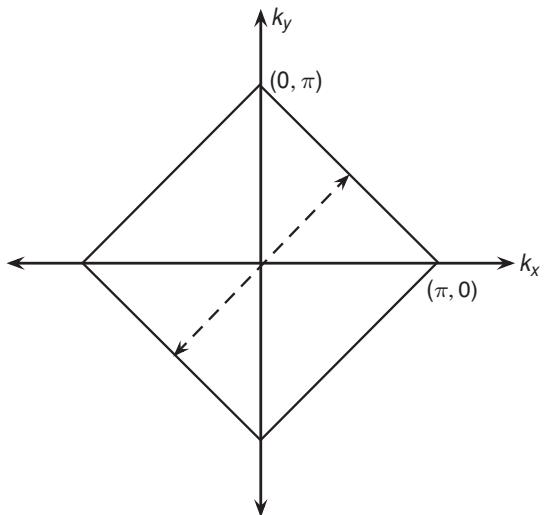
\includegraphics[width=0.50\textwidth]{figs/ch16/fig_16.6.jpg}
\caption*{图 16.6\quad 方晶格上半填充能带的费米面。虚线是嵌套矢量 $(\pi,\pi)$。}\label{fig:auto:16.6}
\end{figure}

我们通过转到动量空间来对角化这个哈密顿量，
\begin{align*}
H^{\mathrm{HF}}_{\text{N\'{e}el}}&=E_{0}+\sum_{\mathbf{k}\in \mathrm{rBZ},\sigma}\epsilon_{\mathbf{k}}\left(c^{\dagger}_{\mathbf{k}A\sigma}c_{\mathbf{k}B\sigma}+c^{\dagger}_{\mathbf{k}B\sigma}c_{\mathbf{k}A\sigma}\right)\\
&+U\sum_{\mathbf{k}\in \mathrm{rBZ},\sigma}\left[(\bar{n}+\Omega_{\sigma})c^{\dagger}_{\mathbf{k}A\sigma}c_{\mathbf{k}A\sigma}+(\bar{n}-\Omega_{\sigma})c^{\dagger}_{\mathbf{k}B\sigma}c_{\mathbf{k}B\sigma}\right]\\
&=E_{0}+\sum_{\mathbf{k}\in \mathrm{rBZ},\sigma}\left(c^{\dagger}_{\mathbf{k}A\sigma}\;\,c^{\dagger}_{\mathbf{k}B\sigma}\right)\\
&\quad\times\begin{pmatrix}U(\bar{n}+\Omega_{\sigma}) & \epsilon_{k}\\ \epsilon_{k} & U(\bar{n}-\Omega_{\sigma})\end{pmatrix}\begin{pmatrix}c_{\mathbf{k}A\sigma}\\ c_{\mathbf{k}B\sigma}\end{pmatrix},\tag{16.64}
\end{align*}
其中 $\epsilon_{\mathbf{k}}=-2t(\cos k_{x}+\cos k_{y})$。对这个简单的能带结构，$\epsilon_{\mathbf{k}}=-\epsilon_{\mathbf{k}+\pi}$。因此 $(\pi,\pi)$ 是嵌套矢量。对角化之后，我们得到两条二重自旋简并的能带，色散为
\begin{equation*}
\omega^{\pm}_{\mathbf{k}}(\bar{n},\Omega)=U\bar{n}\pm\sqrt{U^{2}\Omega^{2}+\epsilon^{2}_{\mathbf{k}}}.\tag{16.65}
\end{equation*}
也就是说，系统中存在一个能隙，而且它完全来自有序化。正如我们将看到的，这类绝缘体与能带绝缘体完全相同，与莫特型绝缘体毫无共同之处。注意 $\epsilon_{\mathbf{k}}=0$ 沿约化 BZ 的边缘 $|k_{x}|+|k_{y}|=\pi$。因此，只有当 $\Omega=0$ 时激发才沿区边缘无能隙。每对平行的边由单个动量 $(\pi,\pi)$ 或 $(\pi,-\pi)$ 相连，这正是方晶格上完美嵌套所预期的，如图 16.6 所描绘。由于上、下两条能带关于能级 $U\bar{n}$ 对称，半填充时下能带应当被完全填满。

由此得到的经典能量密度为
\begin{equation*}
E(\bar{n},\Omega)=U(-\bar{n}^{2}+\Omega^{2})+\frac{2}{N}\sum_{\mathbf{k}\in \mathrm{rBZ}}\omega^{-}_{\mathbf{k}}(\bar{n},\Omega),\tag{16.66}
\end{equation*}
其中第一项是 $E_{0}$，第二项前面的因子 2 来自对自旋的求和。这个平均场计算的自洽条件由对两个变分参数 $\bar{n}$ 与 $\Omega$ 极小化能量
\begin{equation*}
\frac{\partial}{\partial\bar{n}}E=0,\qquad\frac{\partial}{\partial\Omega}E=0,\tag{16.67}
\end{equation*}
来确定。因为 $\partial\omega^{-}_{\mathbf{k}}/\partial\bar{n}=U$ 且 $\partial E_{0}/\partial\bar{n}=-2\bar{n}U$，得 $\bar{n}=1/2$。由第二个条件得到
\begin{equation*}
\Omega=\frac{1}{N}\sum_{\mathbf{k}\in \mathrm{rBZ}}\frac{1}{\sqrt{1+(\epsilon_{\mathbf{k}}/U\Omega)^{2}}}.\tag{16.68}
\end{equation*}
在计算式 (16.68) 中的求和时，使用规则
\begin{equation*}
\frac{1}{N}\sum_{\mathbf{k}\in \mathrm{BZ}}\to\frac{1}{V_{\mathrm{BZ}}}\int_{\mathrm{BZ}}\mathrm{d}^{d}\mathbf{k}\tag{16.69}
\end{equation*}
把求和化为积分是便利的，其中 $V_{\mathrm{BZ}}$ 是布里渊区的体积。意识到我们的求和只在约化布里渊区上进行，我们把 $\Omega$ 化为
\begin{equation*}
\Omega=\frac{1}{(2\pi)^{2}}\int_{|k_{x}|+|k_{y}|\le\pi}\frac{\mathrm{d}k_{x}\mathrm{d}k_{y}}{\sqrt{1+\left[\frac{2t}{U\Omega}(\cos k_{x}+\cos k_{y})\right]^{2}}}.\tag{16.70}
\end{equation*}
作变量代换 $h_{x}=(k_{x}+k_{y})/2$、$h_{y}=(k_{y}-k_{x})/2$（它同时旋转并缩放了积分区域），我们得到
\begin{align*}
\Omega&=\frac{1}{4\pi^{2}}\int_{-\pi/2}^{\pi/2}\mathrm{d}h_{x}\int_{-\pi/2}^{\pi/2}\mathrm{d}h_{y}\frac{|\partial(k_{x},k_{y})/\partial(h_{x},h_{y})|}{\sqrt{1+\left(\frac{2t}{U\Omega}\left(\cos(h_{x}+h_{y})+\cos(h_{y}-h_{x})\right)\right)^{2}}}\\
&=\frac{2}{\pi^{2}}\int_{0}^{\pi/2}\mathrm{d}h_{x}\int_{0}^{\pi/2}\mathrm{d}h_{y}\frac{1}{\sqrt{1+\left(\frac{4t}{U\Omega}\cos h_{x}\cos h_{y}\right)^{2}}}.\tag{16.71}
\end{align*}
在 $t/U\ll 1$ 极限下，按 $t/(U\Omega)$ 的幂展开，我们近似被积函数为
\begin{equation*}
\frac{1}{\sqrt{1+(\epsilon_{\mathbf{k}}/(U\Omega))^{2}}}=1-\frac{1}{2}\left(\frac{4t}{U\Omega}\right)^{2}\cos^{2}h_{x}\cos^{2}h_{y}+O(t/U)^{4},\tag{16.72}
\end{equation*}
这个展开中隐含的一个假定是 $t/U\Omega\ll 1$，而不仅仅是 $t/U\ll 1$。把展开积分到一阶，得到
\begin{equation*}
\Omega=\frac{1}{2}\left(1-2\left(\frac{t}{U}\right)^{2}\frac{1}{\Omega^{2}}+O(t/U)^{4}\right),\tag{16.73}
\end{equation*}
这表明量子涨落会削弱有序的倾向。

为求出领头修正，令 $\Omega=\frac{1}{2}-\epsilon$，得到
\begin{equation*}
\epsilon=\frac{4(t/U)^{2}}{1-16(t/U)^{2}}\simeq 4\left(\frac{t}{U}\right)^{2}.\tag{16.74}
\end{equation*}
值得注意的是，这个结果满足先前的内含假定 $t/U\ll\Omega$。对能量密度，小 $t/U$ 展开给出
\begin{align*}
&E(\bar{n}=\tfrac{1}{2},\Omega)=U\left(\Omega^{2}-\frac{1}{4}\right)\\
&\quad+\frac{2U\Omega}{\pi^{2}}\int_{0}^{\pi/2}\mathrm{d}h_{x}\mathrm{d}h_{y}\left(\frac{1}{2\Omega}-\sqrt{1+\left(\frac{4t}{U\Omega}\cos h_{x}\cos h_{y}\right)^{2}}\right)\\
&\quad=U\left(\Omega^{2}-\frac{1}{4}\right)\\
&\quad+\frac{2U\Omega}{\pi^{2}}\int\mathrm{d}h_{x}\mathrm{d}h_{y}\left[\frac{1}{2\Omega}-1-\frac{1}{2}\left(\frac{4t}{U\Omega}\right)^{2}\cos^{2}h_{x}\cos^{2}h_{y}+O(t/U\Omega)^{4}\right]\\
&\quad=U\left[\left(\Omega^{2}-\frac{1}{4}\right)+\Omega\left(\frac{1}{4\Omega}-\frac{1}{2}-\frac{t^{2}}{U^{2}\Omega^{2}}\right)\right].\tag{16.75}
\end{align*}
代入序参量的结果 $\Omega=\frac{1}{2}-4\left(\frac{t}{U}\right)^{2}$，我们发现基态能量为 $E=-4\frac{t^{2}}{U}$。对哈伯德模型作微扰的 $t/U$ 展开，对半填充哈伯德带的自旋部分也给出同样的结果。然而，由于哈特里--福克近似中严格没有相互作用，无论大 $t/U$ 还是小 $t/U$ 极限与强、弱耦合的对应都完全是启发性的。

现在考虑相反的区域 $t/U\gg 1$。在这个极限下，我们把 $\cos h_{x}$ 在积分上限附近线性化，并用 $\langle\cos h_{y}\rangle=1/2$ 替换 $\cos h_{y}$，从而近似该积分。于是得到
\begin{equation*}
\Omega=\frac{1}{\pi}\int_{0}^{\pi/2}\frac{\mathrm{d}h_{x}}{\sqrt{1+\frac{8}{U^{2}\Omega^{2}}h_{x}^{2}}}=\frac{1}{\alpha\pi}\sinh^{-1}\frac{\alpha\pi}{2},\tag{16.76}
\end{equation*}
其中 $\alpha=\frac{4\sqrt{2}t}{U\Omega}$。解出 $\Omega$，我们得到指数压低的解
\begin{equation*}
\Omega=\frac{2\sqrt{2}\pi\frac{t}{U}}{\sinh(4\sqrt{2}\pi\frac{t}{U})}\sim 4\sqrt{2}\pi\frac{t}{U}\mathrm{e}^{-4\sqrt{2}\pi\frac{t}{U}}\ll 1.\tag{16.77}
\end{equation*}
因此我们发现，无论 $t/U$ 的大小如何，反铁磁序都会在单粒子谱中打开一个能隙。然而，在两种情形中出现的都是非相互作用的哈密顿量。因此，尽管相应的单粒子格林函数依赖于电子填充数，每条能带的权重却不然。它保持为常数，正如能带绝缘体问题中那样。由这一分析得到的信息是清楚的：如果实验体系显示出能隙尺度上的谱权重转移，那么哈特里--福克反铁磁性便不足以解释这些物理。剩下的、尚待解释的部分就是我们所说的 Mott 性。

\subsection{海森堡：$t/U$ 微扰论}

平均场理论的最终目标，是用一个由二次型哈密顿量描述的更简单的系统为相互作用的系统建模。这只能通过某种方式解耦四费米子相互作用来实现。自然产生的问题是：什么时候解耦一个四费米子项并用某种有序倾向来替换它才是合法的？既然只有存在相互作用时才可能有有序化，平均场理论并不直接与弱耦合挂钩。它只是断言：无论大小如何，相互作用导致有序化。然而，在哈伯德模型中存在两种不同的产生反铁磁有序的机制。除了基于费米面嵌套的平均场机制之外，还存在一种强耦合类比，其中局域物理导致电子自旋的交错有序。这两种机制是彼此不同的。为确立后者，在强耦合区域 $t/U\ll 1$ 中围绕原子极限作展开、导出一个有效哈密顿量即可。在这个极限下，可以微扰地发展出一个有效哈密顿量，并可以证明它有利于反铁磁性。实现这类计算有若干种方式。强耦合展开的首要目标，是使哈伯德模型相对于原子极限中的大能量尺度 $U$ 成为块对角形式。于是，低能模型将对应于在无双占据分部中运作的哈密顿量。然而，这种消除双占据的变换会不加区分地混合原来的原子态，无论其占据情况如何。

\subsection*{哈伯德二聚体}

哈伯德模型中的 $t/U$ 展开是简并微扰论的一次演练。哈伯德模型的任何本征态都可以写成
\begin{equation*}
|\psi\rangle=a_{0}|\psi_{0}\rangle+a_{1}|\psi_{1}\rangle+\cdots=\sum_{m}a_{m}|\psi_{m}\rangle\tag{16.78}
\end{equation*}
这样的项之和，其中每一项具有确定数目的双占据格点，$|\psi_{m}\rangle$。各个 $|\psi_{m}\rangle$ 是原子极限（$t=0$）下的本征态。在这个极限下，保持 $m$ 不变的局域占据方式有很多种，因而简并度很大。从式 (16.78) 可以清楚看到：哈伯德模型没有哪个本征态具有固定的双占据格点数。考虑两个格点、两个电子（一个自旋向上、一个自旋向下）的系统。天真地看，这个系统的基态被预期为单态：
\begin{equation*}
|\psi_{\mathrm{S}}\rangle=\frac{1}{\sqrt{2}}\left(|\uparrow,\downarrow\rangle-|\downarrow,\uparrow\rangle\right).\tag{16.79}
\end{equation*}
然而 $|\psi_{\mathrm{S}}\rangle$ 并不是哈伯德模型的本征态。真正归一化的基态
\begin{equation*}
|\psi_{2\text{-site}}\rangle=\frac{\alpha}{\sqrt{2(\alpha^{2}+1)}}\left(|\uparrow,\downarrow\rangle-|\downarrow,\uparrow\rangle+\alpha^{-1}|0,2\rangle-\alpha^{-1}|2,0\rangle\right),\tag{16.80}
\end{equation*}
含有与双占据分部（$|0,2\rangle\equiv|0,\uparrow\downarrow\rangle$）的混合，混合系数为 $\alpha=4t/(-U+\sqrt{16t^{2}+U^{2}})\approx 2U/t$\footnote{译注：按前一式严格展开，小 $t/U$ 时应为 $\alpha\approx U/(2t)$，原文印作 $2U/t$。}，因而 $\alpha^{-1}$ 在 $U=\infty$ 时消失。结果，对任何有限的 $U$，与双占据分部的混合甚至存在于基态之中。无论填充和系统大小如何，这一特征都显而易见。

\subsection*{相似变换}

哈伯德二聚体的例子表明，真正的低能基态与所有原子态都有非零混合，无论其能量高低。在这个意义上，设想通过移走裸电子态的双占据来获得低能理论是一种误解。不过，在某种意义上，微扰论做的恰恰就是这件事。当哈伯德哈密顿量被化成块对角形式时，使之成为可能的算符对应于多粒子电子态的混合。正是相对于这些算符，哈伯德模型中的各个块才保持双占据格点的数目。让我们定义（[E1994; C2004]）$f_{i\sigma}$ 来表示使哈伯德模型块对角化的变换后的费米子，也就是说，$f_{i\sigma}$ 保持双占据格点的数目。对任意算符 $O$，我们定义 $\tilde{O}$ 使得
\begin{equation*}
O\equiv\mathbf{O}(c),\qquad\tilde{O}\equiv\mathbf{O}(f),\tag{16.81}
\end{equation*}
即简单地把费米算符 $c_{i\sigma}$ 替换为变换后的费米子 $f_{i\sigma}$。例如
\begin{equation*}
\tilde{V}=U\sum_{i}\tilde{n}_{i\uparrow}\tilde{n}_{i\downarrow}=U\sum_{i}f^{\dagger}_{i\uparrow}f_{i\uparrow}f^{\dagger}_{i\downarrow}f_{i\downarrow}.\tag{16.82}
\end{equation*}
正如我们将显式看到的，$O$ 与 $\tilde{O}$ 仅在 $U=\infty$ 时才等价。

使哈伯德模型块对角化的流程如今已广为人知（[E1994; C2004]）。人们构造一个相似变换 $S$，它连接至多相差一个“虚拟”双占据格点的分部，使得原来的哈伯德模型
\begin{equation*}
H=\mathrm{e}^{S}\tilde{H}\mathrm{e}^{-S},\tag{16.83}
\end{equation*}
满足对易关系
\begin{equation*}
[H,\tilde{V}]=0,\tag{16.84}
\end{equation*}
这意味着变换后费米子的双占据是好量子数，所有本征态都可以据此标记。在基态中 $\tilde{V}=0$，且
\begin{equation*}
f_{i\uparrow}f_{i\downarrow}|\mathrm{GS}\rangle=0.\tag{16.85}
\end{equation*}
这将帮助我们组织微扰论。注意，变换后的哈密顿量并不满足 $[\tilde{H},V]=0$。为组织微扰论，我们对式 (16.17) 中动能项的各个贡献引入算符 $\tilde{T}_{m}$。$\tilde{T}_{m}$ 使双占据格点的数目增加 $m$。由式 (16.17) 有
\begin{align*}
\tilde{T}_{0}=-t\sum_{\langle ij\rangle}\left(\tilde{\eta}^{\dagger}_{i\sigma}\tilde{\eta}_{j\sigma}+\tilde{\xi}^{\dagger}_{i\sigma}\tilde{\xi}_{j\sigma}\right),\\
\tilde{T}_{1}=-t\sum_{\langle ij\rangle}\tilde{\eta}^{\dagger}_{i\sigma}\tilde{\xi}_{j\sigma},\tag{16.86}
\end{align*}
且 $\tilde{T}_{-1}=\tilde{T}^{\dagger}_{1}$。由于每个 $\tilde{T}_{m}$ 使双占据格点数目增加 $m$，一个简单的对易关系
\begin{equation*}
[\tilde{V},\tilde{T}_{m}]=mU\tilde{T}_{m},\tag{16.87}
\end{equation*}
支配着动能项与势能项的各个贡献。哈密顿量 $\tilde{H}$ 包含变换后的动能项 $\tilde{T}_{0}+\tilde{T}_{-1}+\tilde{T}_{1}$。后两项必须被消去，因为它们不保持双占据格点的数目。在微扰论中逐阶地找到满足式 (16.84) 的 $S$ 是可能的。展开式 (16.83)，我们发现最低阶项满足
\begin{equation*}
H=\tilde{V}+\tilde{T}_{0}+\tilde{T}_{-1}+\tilde{T}_{1}+[S^{(1)},\tilde{V}+\tilde{T}_{0}+\tilde{T}_{-1}+\tilde{T}_{1}].\tag{16.88}
\end{equation*}
我们定义 $S^{(1)}$ 为
\begin{equation*}
\tilde{T}_{1}+\tilde{T}_{-1}+[S^{(1)},\tilde{V}]=0\tag{16.89}
\end{equation*}
的解。利用式 (16.87)，我们发现
\begin{equation*}
S^{(1)}=\frac{1}{U}\left(\tilde{T}_{1}-\tilde{T}_{-1}\right).\tag{16.90}
\end{equation*}
于是，我们的变换后哈密顿量变为
\begin{equation*}
H=\tilde{V}+\tilde{T}_{0}+[\tilde{T}_{1},\tilde{T}_{-1}]\frac{1}{U}+[\tilde{T}_{1}-\tilde{T}_{-1},\tilde{T}_{0}]\frac{1}{U}+\cdots.\tag{16.91}
\end{equation*}
最后一项含与 $\tilde{T}_{0}$ 的对易子，不保持双占据格点的数目。它可以通过相似变换
\begin{equation*}
S^{(2)}=[\tilde{T}_{1}+\tilde{T}_{-1},\tilde{T}_{0}]\frac{1}{U^{2}},\tag{16.92}
\end{equation*}
在二阶上消去。就我们的讨论而言，我们将只保留有效哈密顿量中到 $t/U$ 二阶的项。于是，我们的哈密顿量到 $O(t^{2}/U)$ 为
\begin{equation*}
H=\tilde{V}+\tilde{T}_{0}+[\tilde{T}_{1},\tilde{T}_{-1}]\frac{1}{U},\tag{16.93}
\end{equation*}
其中只含 $\tilde{T}_{m}$ 诸项指标之和为零的项。这个哈密顿量中出现的对易子，除非 $\tilde{T}_{1}$ 与 $\tilde{T}_{-1}$ 含有共同指标，否则为零。我们的哈密顿量描述的是哈密顿量中 $\tilde{V}$ 取确定值的任意块内的输运。回想 $\tilde{T}_{0}$ 的一部分严格在上哈伯德带（UHB）内搬运电荷。如果我们只想描述能量最低的分部，就要消去所有要求 $\tilde{V}\neq 0$ 的项。这可以通过把哈密顿量投影到无双占据分部来实现：
\begin{equation*}
P_{0}HP_{0}=-t\sum_{\langle ij\rangle}\tilde{\xi}^{\dagger}_{i\sigma}\tilde{\xi}_{j\sigma}-\frac{1}{U}\tilde{T}_{-1}\tilde{T}_{1},\tag{16.94}
\end{equation*}
其中默认 $\tilde{T}_{m}$ 诸算符共享一个共同指标。我们进一步简化，注意到第二项中存在两种不同类型的相互作用，即两格点项与三格点项。考虑只含相邻格点的两格点项。直接代入式 (16.86) 表明，$\tilde{T}_{-1}\tilde{T}_{1}$ 中唯一非零的最近邻项形如
\begin{equation*}
\left(\tilde{T}_{-1}\tilde{T}_{1}\right)_{2\text{-site}}=t^{2}\sum_{i,j,\sigma}\tilde{\xi}^{\dagger}_{i\sigma}\tilde{\eta}_{i+j\sigma}\tilde{\eta}^{\dagger}_{i+j\sigma'}\tilde{\xi}_{i\sigma'}.\tag{16.95}
\end{equation*}
这一项或者在相邻格点之间把一个自旋向上转换为自旋向下，或者保持自旋组态不变。因此，示意性地它形如
\begin{align*}
\sum_{\sigma,\sigma'}\tilde{\xi}^{\dagger}_{i\sigma}\tilde{\eta}_{j\sigma}\tilde{\eta}^{\dagger}_{j\sigma'}\tilde{\xi}_{i\sigma'}=\sum_{\sigma}|\sigma_{i},\bar{\sigma}_{j}\rangle\langle\sigma_{i},\bar{\sigma}_{j}|+|\sigma_{i},\bar{\sigma}_{j}\rangle\langle\bar{\sigma}_{i},\sigma_{j}|\\
=\sum_{\sigma}(1-\tilde{n}_{i\bar{\sigma}})\tilde{n}_{i\sigma}\tilde{n}_{j\bar{\sigma}}(1-\tilde{n}_{j\sigma})-\tilde{c}^{\dagger}_{i\sigma}\tilde{c}_{i\bar{\sigma}}\tilde{c}^{\dagger}_{j\bar{\sigma}}\tilde{c}_{j\sigma}.\tag{16.96}
\end{align*}
另一方面，自旋--自旋相互作用项 $\mathbf{S}_{i}\cdot\mathbf{S}_{j}$ 可以写成
\begin{equation*}
\mathbf{S}_{i}\cdot\mathbf{S}_{j}=\sum_{\sigma}\frac{1}{2}\tilde{c}^{\dagger}_{i\sigma}\tilde{c}_{i\bar{\sigma}}\tilde{c}^{\dagger}_{j\bar{\sigma}}\tilde{c}_{j\sigma}+\frac{1}{4}(\tilde{n}_{i\sigma}\tilde{n}_{j\sigma}-\tilde{n}_{i\sigma}\tilde{n}_{j\bar{\sigma}}).\tag{16.97}
\end{equation*}
第一项代表 $S^{+}_{i}S^{-}_{j}+S^{-}_{i}S^{+}_{j}$，第二项表示 $S^{z}_{i}S^{z}_{j}$。把后者代入式 (16.96)，我们得到
\begin{equation*}
-\frac{t^{2}}{U}\sum_{\sigma,\sigma',\langle ij\rangle}\tilde{\xi}^{\dagger}_{i\sigma}\tilde{\eta}_{j\sigma}\tilde{\eta}^{\dagger}_{j\sigma'}\tilde{\xi}_{i\sigma'}=\frac{2t^{2}}{U}\sum_{\langle ij\rangle}\mathbf{S}_{i}\cdot\mathbf{S}_{j}-H_{2}\tag{16.98}
\end{equation*}
作为涉及最近邻格点的相互作用项的工作表达式，其中
\begin{equation*}
H_{2}=\frac{t^{2}}{U}\sum_{\langle ij\rangle\sigma}\left[\frac{1}{2}(\tilde{n}_{i\sigma}\tilde{n}_{j\sigma}+\tilde{n}_{i\sigma}\tilde{n}_{j\bar{\sigma}})+(1-\tilde{n}_{i\bar{\sigma}})\tilde{n}_{i\sigma}\tilde{n}_{j\bar{\sigma}}(1-\tilde{n}_{j\sigma})\right].\tag{16.99}
\end{equation*}
三格点跳跃项来自 $\tilde{\xi}^{\dagger}_{i+\delta\sigma}\tilde{\eta}_{i\sigma}\tilde{\eta}^{\dagger}_{i\sigma'}\tilde{\xi}_{i+\delta'\sigma'}$，并约化为
\begin{align*}
H_{3}\equiv-t^{2}/U\sum_{\sigma,\sigma',i,\delta,\delta'}\Big[(1-\tilde{n}_{i+\delta,\bar{\sigma}})f^{\dagger}_{i+\delta,\sigma}\tilde{n}_{i\bar{\sigma}}(1-\tilde{n}_{i\sigma})f_{i+\delta',\sigma}(1-\tilde{n}_{i+\delta',\bar{\sigma}})\\
-(1-\tilde{n}_{i+\delta,\sigma})f^{\dagger}_{i+\delta,\bar{\sigma}}f^{\dagger}_{i,\sigma}f_{i\bar{\sigma}}f_{i+\delta',\sigma}(1-\tilde{n}_{i+\delta',\bar{\sigma}})\Big].\tag{16.100}
\end{align*}
于是，能量最低分部中的哈密顿量为
\begin{equation*}
H_{\mathrm{LHB}}=P_{0}HP_{0}=H_{t-J}-H_{2}+H_{3}\tag{16.101}
\end{equation*}
其中
\begin{equation*}
H_{t-J}=-t\sum_{\langle ij\rangle}\tilde{\xi}^{\dagger}_{i\sigma}\tilde{\xi}_{j\sigma}+2\frac{t^{2}}{U}\sum_{\langle ij\rangle}\mathbf{S}_{i}\cdot\mathbf{S}_{j}\tag{16.102}
\end{equation*}
正是研究空穴掺杂哈伯德模型时常用的 $t$--$J$ 极限。$H_{2}$ 与 $H_{3}$ 两项清楚地表明，$t$--$J$ 模型并不是哈伯德模型真正的低能极限。事实上，在半填充时断言 $t$--$J$ 模型是哈伯德模型的低能理论会带来一个问题。由于自旋算符可以用
\begin{equation*}
\Psi=\begin{pmatrix}f_{\uparrow} & f_{\downarrow}\\ f^{\dagger}_{\downarrow} & -f^{\dagger}_{\uparrow}\end{pmatrix},\tag{16.103}
\end{equation*}
写成 $\mathbf{S}=\frac{1}{2}\mathrm{Tr}\,\Psi^{\dagger}\Psi\sigma^{\mathrm{T}}$，$t$--$J$ 模型在半填充时具有一个附加的对称性。半填充（每格点一个电子）时，动能项消失。结果，$t$--$J$ 模型完全约化为一个自旋--自旋模型，即海森堡模型，其基态能量恰好是我们由哈特里--福克拟设计算出的 $-4t^{2}/U$。然而，海森堡模型比哈伯德模型具有更高的对称性（[DFM1988; AZ1988]）。具体地说，若令 $\Psi\to h\Psi$，其中 $h$ 是形如
\begin{equation*}
h=\begin{pmatrix}a_{1} & b_{1}\\ -b^{*}_{1} & a^{*}_{1}\end{pmatrix}\tag{16.104}
\end{equation*}
的 $SU(2)$ 矩阵，$|a_{1}|^{2}+|b_{1}|^{2}=1$，则每个自旋算符 $S$ 保持不变，因为
\begin{equation*}
\Psi^{\dagger}\Psi\to\Psi^{\dagger}h^{\dagger}h\Psi=\Psi^{\dagger}\Psi.\tag{16.105}
\end{equation*}
因此，每个自旋都可以独立于其他自旋转动。在完整的哈伯德模型中，所有自旋必须以完全相同的方式转动才能保持哈密顿量不变，也就是说，只有整体 $SU(2)$ 对称性：$\Psi\to\Psi g$，其中 $g$ 是一个 $SU(2)$ 矩阵。虽然在对 $f_{i\sigma}$ 费米子而言的无双占据变换基中，$H_{3}$ 在半填充时严格为零，$H_{2}$ 却不然。$H_{2}$ 中的第二项破坏了 $t$--$J$ 极限在半填充时的局域 $SU(2)$ 对称性，只留下哈伯德模型的整体 $SU(2)$ 对称性。

在这一点上，用原来的电子算符重新表达我们约化后的哈密顿量是有益的。这样做，我们将能更清楚地从电子算符的角度看出，为什么 $t$--$J$ 模型在半填充时的局域 $SU(2)$ 对称性被约化为整体 $SU(2)$ 对称性。为此，我们需要变换电子算符。由算符 $O$ 的一般变换
\begin{equation*}
O=\mathrm{e}^{S}\tilde{O}\mathrm{e}^{-S}=\tilde{O}+[S,\tilde{O}]+\frac{1}{2!}[S,[S,O]]+\cdots,\tag{16.106}
\end{equation*}
代入式 (16.90)，我们得到一个直到 $O(t/U)$ 都有效的表达式
\begin{equation*}
O=\tilde{O}+\frac{1}{U}[\tilde{T}_{1}-\tilde{T}_{-1},\tilde{O}]+\cdots,\tag{16.107}
\end{equation*}
由于 $S$ 连接相差一个双占据格点的分部，算符 $O$ 生活在哈伯德模型的完整希尔伯特空间中。尽管如此，我们仍可以得到任何算符完全处于能量最低分部中的展开，因为 $\tilde{O}$ 算符可以分解为产生或湮灭特定数目双占据格点的部分。也就是说，我们把变换后的算符分解为
\begin{equation*}
\tilde{O}=\sum_{n\in\mathbb{Z}}\tilde{O}_{nU}.\tag{16.108}
\end{equation*}
作为一个简单的例子，考虑变换后的电子湮灭算符
\begin{equation*}
f_{i\sigma}=f_{i\sigma;0}+f_{i\sigma;-U},\tag{16.109}
\end{equation*}
其中 $f_{i\sigma;0}=\tilde{\xi}_{i\sigma}$，$f_{i\sigma;-U}=\tilde{\eta}_{i\sigma}$。注意，对裸费米子算符类似的改写行不通；也就是说，$c_{i\sigma;0}\neq\xi_{i\sigma}$，因为这些算符顾及的是哈伯德模型的完整希尔伯特空间。尽管如此，利用 $f_{i\sigma}$ 算符的可分解性，我们可以借助式 (16.107) 为 $c_{i\sigma;0}$ 建立一个展开。我们只需保证所有对易子中的指标之和为零，如习题 16.4 所示。于是我们得到
\begin{equation*}
c_{i\sigma;0}=\tilde{\xi}_{i\sigma}+\frac{1}{U}[\tilde{T}_{1},\tilde{\eta}_{i\sigma}]+\cdots=\tilde{\xi}_{i\sigma}-\frac{1}{U}\eta_{i\sigma}\tilde{T}_{1}+\cdots.\tag{16.110}
\end{equation*}
最后一步的简化源于：对空穴掺杂而言，变换后的费米子没有双占据。这类表达式将在后面一节中用来导出下哈伯德带的谱权重。但从这个表达式已经可以清楚看到，谱权重含有 $t/U$ 分量，因而并不严格等于 $1+x$。当我们讨论动力学谱权重转移时，这一点将被凸显出来。

然而，我们当前的目标，是用生活在哈伯德模型完整希尔伯特空间中的裸电子算符来重新表达哈密顿量的 $t/U$ 展开。这可以做到：直接把正则变换作用于电子算符并保留所有的项，而不是像式 (16.110) 中那样只保留保持哈伯德模型中某个特定块的能量的项。利用式 (16.107)，我们发现
\begin{equation*}
\xi_{i\sigma}=\tilde{\xi}_{i\sigma}+\frac{1}{U}[\tilde{T}_{1}-\tilde{T}_{-1},\tilde{\xi}_{i\sigma}]+O(t/U)^{2}.\tag{16.111}
\end{equation*}
每个对易子都可以借助
\begin{equation*}
[AB,C]=A\{B,C\}-\{A,C\}B\tag{16.112}
\end{equation*}
以及式 (16.90) 中的反对易关系来简化。不出所料，结果
\begin{equation*}
\begin{aligned}
\xi_{i\sigma}={}&\tilde{\xi}_{i\sigma}-\frac{t}{U}\sum_{j}g_{ij}\big[(1-\tilde{n}_{i\bar{\sigma}})\tilde{n}_{j\bar{\sigma}}f_{j\sigma}\\
&+f^{\dagger}_{i\bar{\sigma}}f_{i\sigma}\tilde{n}_{j\sigma}f_{j\bar{\sigma}}-(1-\tilde{n}_{j\sigma})f^{\dagger}_{j\bar{\sigma}}f_{i\sigma}f_{i\bar{\sigma}}\big]+O(t/U)^{2},
\end{aligned}\tag{16.113}
\end{equation*}
是转动空间中多粒子态的线性组合。$\xi_{i\sigma}$ 与式 (16.110) 的关键区别在于：前者挑出所有单占据格点，而后者只计入最低能带中的单占据格点。$\xi_{i\sigma}$ 的表达式可以求逆，使得 $\tilde{\xi}_{i\sigma}$
\begin{equation*}
\begin{aligned}
\tilde{\xi}_{i\sigma}={}&\xi_{i\sigma}+\frac{t}{U}\sum_{j}g_{ij}\big[(1-n_{i\bar{\sigma}})n_{j\bar{\sigma}}c_{j\sigma}\\
&+c^{\dagger}_{i\bar{\sigma}}c_{i\sigma}n_{j\sigma}c_{j\bar{\sigma}}-(1-n_{j\sigma})c^{\dagger}_{j\bar{\sigma}}c_{i\sigma}c_{i\bar{\sigma}}\big]+O(t/U)^{2},
\end{aligned}\tag{16.114}
\end{equation*}
用裸电子算符表出。所有正比于 $t/U$ 的项都显式地涉及双占据。因此，只有当 $U=\infty$ 时才有 $\tilde{\xi}_{i\sigma}=\xi_{i\sigma}$。正是这些 $t/U$ 修正把对称性恢复到恰为哈伯德模型的整体 $SU(2)$ 对称性。为看清这一点，我们只需把式 (16.114) 代入 $H_{2}$ 与 $H_{3}$。注意，由于 $\tilde{\xi}_{i\sigma}$ 存在 $t/U$ 修正，动能项中会产生正比于 $t^{2}/U$ 的新相互作用。这些项与自旋物理毫无关系，但会显式地涉及双占据，正如下面所看到的：
\begin{align*}
H_{\mathrm{LHB}}&=\mathrm{e}^{-S}P_{0}\mathrm{e}^{S}H\mathrm{e}^{-S}P_{0}\mathrm{e}^{S}\\
&=-t\sum_{\langle i,j\rangle}\xi^{\dagger}_{i\sigma}\xi_{j\sigma}-\frac{t^{2}}{U}\sum_{i}b^{(\xi)\dagger}_{i}b^{(\xi)}_{i}\\
&\quad-\frac{t^{2}}{U}\sum_{\langle i,j\rangle,\langle i,k\rangle,\sigma}\left\{\xi^{\dagger}_{k\sigma}\big[(1-n_{i\bar{\sigma}})\eta_{j\sigma}+\xi^{\dagger}_{j\bar{\sigma}}\xi_{i\bar{\sigma}}\eta_{i\sigma}+\xi^{\dagger}_{i\bar{\sigma}}\xi_{i\sigma}\eta_{j\bar{\sigma}}\big]+\mathrm{h.c.}\right\}.\tag{16.115}
\end{align*}
式 (16.115) 末行的第一项代表三格点跳跃过程。末行中的其余各项来自 $H_{2}$，甚至在半填充时也存在。所有这些项
\begin{figure}[H]\centering
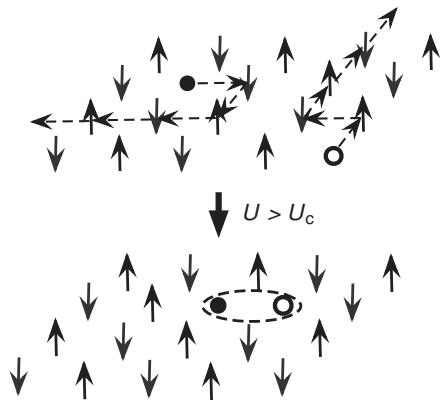
\includegraphics[width=0.52\textwidth]{figs/ch16/fig_16.7.jpg}
\caption*{图 16.7\quad 莫特提出的母体材料（半填充能带）中绝缘态的机制。上（下）箭头表示自旋向上（向下）的电子。当在位相互作用 $U$ 低于临界值时，双占据格点（实心圆点）与空穴（空心圆圈）可以自由输运；当 $U$ 高于临界值时，它们被束缚成局域的对，从而无法导电。}\label{fig:auto:16.7}
\end{figure}

通常都被丢弃。然而我们看到，若对算符作变换，它们便会自然出现，并贡献出与自旋交换项同阶的 $t^{2}/U$ 项。因此，把它们排除在外并没有什么系统性的依据。

\section{动力学谱权重转移}

微扰分析清楚表明，莫特绝缘态并不像原子极限图像让我们相信的那样容易理解。问题在于，双占据显式地出现在基态之中。因此，莫特能隙不能简单地看成到第一个含双占据的态之间的能隙。尽管如此，电荷能隙的判据仍然可以严格表述。如图 16.7 所描绘，双占据会留下一个空格点。这个空格点也许不必再激发到上能带就能自由移动。若果真如此，半填充能带实际上是导体。莫特（[M1949]）在其经典论文中指出了这一点，并论证：要使半填充能带绝缘，空格点与双占据格点之间必须存在某种束缚（见图 16.7）。事实上，此后若干研究者，例如 Kohn（[K1964]）、Fulde（[KHF1982]）以及 Castellani 及其合作者（[C1979]），都指出莫特绝缘体可以看成这样一种态：其中双占据是局域化的，而在导电态中则是退局域化的。因此，莫特转变到局域化状态时所涉及的自由度，并不显式地包含在初始的高能量紫外（UV）完备模型之中。也就是说，莫特能隙是动力学产生的，任何针对莫特体系的单电子描述都是无效的。虽然有序化可以直接从哈伯德模型的弱耦合或强耦合（$t/U$）分析中得到理解，束缚态的形成却不能，因为它从根本上源于基本场的重组。

\begin{figure}[H]\centering
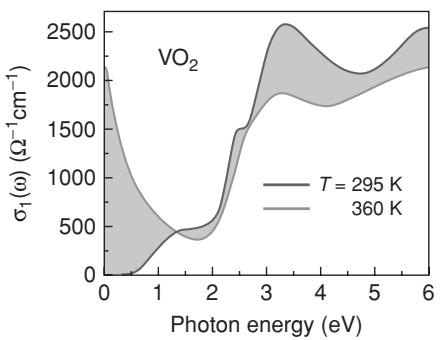
\includegraphics[width=0.48\textwidth]{figs/ch16/fig_16.8_a.jpg}\hfill
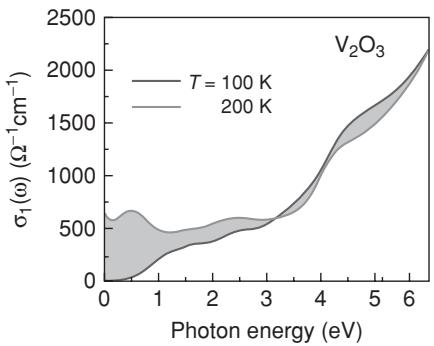
\includegraphics[width=0.48\textwidth]{figs/ch16/fig_16.8_b.jpg}
\caption*{图 16.8\quad $\mathrm{VO}_2$ 与 $\mathrm{V}_2\mathrm{O}_3$ 在莫特绝缘态开始出现的温度之上、之下的光电导（optical conductivity）实部。在 $\mathrm{VO}_2$ 和 $\mathrm{V}_2\mathrm{O}_3$ 中，向绝缘态的转变都伴随着谱权重从化学势附近向远至 6 eV 处的态的转移。这种向莫特态转变时谱权重的大规模重组是莫特转变的普遍特征。数据翻印自 Qazilbash 等，Phys. Rev. B 77, 115121 (2008)。}\label{fig:auto:16.8}
\end{figure}

它标志着微扰论的失效，正如我们在近藤问题中已经看到的那样——低温下的自由度是初始哈密顿量中并不存在的束缚态。

正如上一节所见，莫特绝缘体的特征是单粒子电子格林函数沿动量空间中一个连通曲面消失。格林函数实部消失的一个前提是谱函数在化学势上下都必须非零。金属中，谱权重位于化学势附近。于是问题来了：能隙一旦打开，原本处于化学势处的谱权重到哪里去了？它是像平均场理论中那样被推到恰在能隙之上的态，还是在远远超过能隙的能量处重新出现？这个问题的答案直指莫特问题的核心。考虑经典的莫特体系 $\mathrm{VO}_2$，它在 340 K 以下转变为绝缘态。在该体系中，每个钒离子的价为 $+4$，给出半填充的 $d^{1}$ 组态。$\mathrm{VO}_2$ 的特别之处在于，它直到最低温度都不发生磁有序。然而，伴随而来的结构重排使强关联的作用变得模糊。随温度降低跨过转变时，结构从高度对称的四方金红石结构变为单斜结构，其中钒原子发生二聚化并相对 $c$ 轴倾转。此外，载流子密度（[G1971]）从高温下的 $10^{23}\,\mathrm{cm}^{-3}$ 降到低温下的 $10^{18}\,\mathrm{cm}^{-3}$。结果，$\mathrm{VO}_2$ 中出现了与大多数半填充能带同样的问题：绝缘态究竟来自对称性破缺，还是如图 16.7 所示的那样完全来自强关联？尽管莫特（[ZM1975; RLP1994]）指出 0.6 eV 的能隙——即 $\mathrm{VO}_2$ 的电荷能隙——超出了钒离子二聚化可能涉及的任何能量尺度，这个问题依然存在。用椭偏法（ellipsometry）探测的该体系的光学响应，在这里对裁决这一问题特别有用。图 16.8 所示的关键特征是：把温度降到 295 K（[Q2008]）——这一能量尺度远小于 0.6 eV——会导致谱权重从化学势附近的态（浅色线）转移到能量高得多的态（深色线），距离约 6 eV 甚至更远。谱权重重新分布所涉及的这些能量尺度远远超过与二聚化相关的尺度；但它们与 $U$ 尺度上的关联物理一致。这就是 Mott 性（Mottness），而且正如我们将看到的，即使转变到超导态，它依然存在。事实上，这种情形甚至在半填充能带中也出现，例如 $\mathrm{V}_2\mathrm{O}_3$，已知（[Q2008]）其绝缘态具有反铁磁有序。图 16.8 的第二个面板给出了 $\mathrm{V}_2\mathrm{O}_3$ 中金属—绝缘体转变时的类似光电导。与 $\mathrm{VO}_2$ 一样，向绝缘态的转变同样涉及谱权重从化学势向至少 6 eV 之外的态的转移。这种高、低能量尺度的混合是莫特体系中的普遍现象。因此，对电荷能隙而言，核心是携带着 $U$ 尺度的传播自由度，而不仅仅是与可能发生的某种有序现象相联系的较小的能量尺度。$\mathrm{VO}_2$ 中另一处奇特之处是，能隙打开的温度远小于能隙本身。事实上，$\mathrm{VO}_2$ 的 $\Delta/T_{\mathrm{MI}}\approx 20$，至少是 BCS 理论中相应比值的 10 倍。

\subsection{掺杂莫特绝缘体：铜氧面}

高温铜氧化物超导体代表了另一类莫特体系，它们表现出以 $\mathrm{VO}_2$ 为典型的同一种紫外—红外（UV--IR）混合。铜氧化物是层状钙钛矿，其活跃层为铜氧面，其电子结构如图 16.9(a) 所示。在与铜氧化物相关的四面体晶体场中，一个未配对电子位于 $d_{x^{2}-y^{2}}$ 轨道上。因此，只考虑哈伯德型的单带模型似乎是很自然的。然而，未掺杂的铜氧化物实际上是如图 16.9(b) 那样的电荷转移绝缘体（charge-transfer insulator）。在这类体系中，每个单胞内不止一个原子，此处是一个氧原子。$d_{x^{2}-y^{2}}$ 轨道与氧的 $p_{x}$、$p_{y}$ 轨道杂化，因而三带模型才是自然的。不过，只要在位排斥能 $U$ 是最大的能量尺度，且单胞内原子之间的杂化足够可观（[ZR1988; MES1993]），约化为单带哈伯德模型就是合理的。铜氧化物正是这种情形。因此，铜氧化物超导电性的秘密至少蕴含在二维哈伯德模型的解中。图 16.10 给出了 $\mathrm{YBa}_2\mathrm{Cu}_3\mathrm{O}_y$ 沿 $\mathrm{CuO}_2$ 面、氧掺杂量分别为 $y=6.1$ 和 $y=6.6$ 时的光电导（[C1990; L2005]）。在很好的近似下，$y=6.1$ 代表母体材料，其频率低于 1.2 eV（铜氧化物的光学能隙）的光吸收受到明显抑制。这与母体绝缘材料中的莫特能隙一致。而在掺杂体系 $y=6.6$ 中，低于 $\approx 1.2\,\mathrm{eV}$ 的光电导强抑制消失了，并伴随高能区（距化学势约 3 eV）谱强度的减小。这种行为类似于 $\mathrm{VO}_2$ 在 340 K 以上向金属态转变时谱权重的反转。事实上，这两个体系中，掺杂诱导的金属态与温度诱导的转变所涉及的能量尺度完全相同。这种发生在 $O(U)$ 能量尺度上的重组只能源于强的电子关联。

\begin{figure}[H]\centering
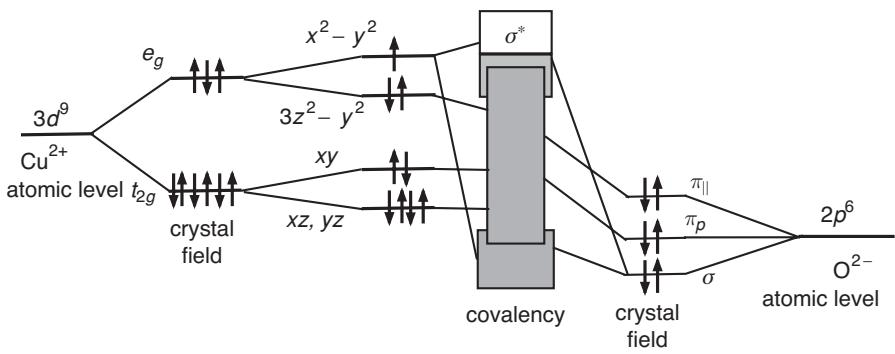
\includegraphics[width=0.8\textwidth]{figs/ch16/fig_16.9_a.jpg}

\vspace{0.5em}
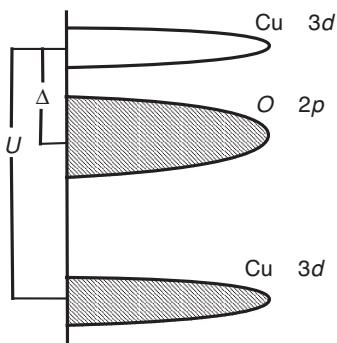
\includegraphics[width=0.42\textwidth]{figs/ch16/fig_16.9_b.jpg}
\caption*{图 16.9\quad 铜氧化物超导体中铜氧面的电子结构。(a) 铜氧面中原子的轨道占据与能级劈裂。上 $d$ 能级为单占据，但材料却是绝缘体，这使关联成为电子性质的主角。(b) 母体材料能带填充的示意描绘。$U$ 是两个电子占据 $\mathrm{d}_{x^{2}-y^{2}}$ 能级时的在位排斥能，$\Delta$ 是氧 $p$ 带与空的 $d$ 能级之间的能隙。在 $U\gg\Delta$ 且杂化足够大的极限下，电荷转移绝缘体可约化为单带哈伯德模型，从而等价于莫特绝缘体。}\label{fig:auto:16.9}
\end{figure}

光电导的探针是电流，因此它应当直接给出载流子总数的指示。正如本章开头所见，引入能带绝缘体或半导体的每个空穴都会在化学势上方产生一个准粒子。那么，在掺杂莫特绝缘体中会发生什么？我们猜想，由于谱权重从谱的高能部分转移过来，准粒子的数目必定超过裸掺杂量。事实正是如此。对光电导作积分，我们可以算出有效载流子数，或更准确地说是归一化载流子密度，
\begin{equation*}
N_{\mathrm{eff}}(\Omega)=\frac{2mV_{\mathrm{cell}}}{\pi e^{2}}\int_{0}^{\Omega}\sigma(\omega)\,\mathrm{d}\omega,\tag{16.116}
\end{equation*}
\begin{figure}[H]\centering
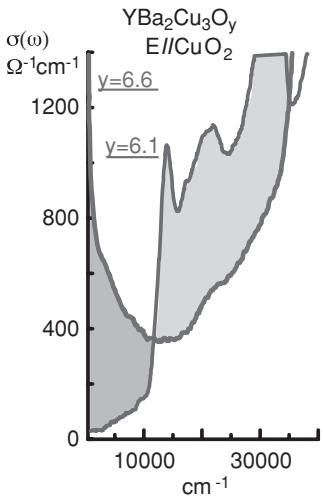
\includegraphics[width=0.32\textwidth]{figs/ch16/fig_16.10.jpg}
\caption*{图 16.10\quad $\mathrm{YBa}_2\mathrm{Cu}_3\mathrm{O}_y$（YBCO）在两个掺杂量下面内光电导的演化。在很好的近似下，$y=6.1$ 代表母体材料，$y=6.6$ 代表过掺杂样品。关键特征是：“母体”材料中 1.2 eV 以上的谱权重在掺杂后转移到化学势附近的态。翻印自 Cooper 等，Phys. Rev. B 47, 8233 (1993)。}\label{fig:auto:16.10}
\end{figure}
\begin{figure}[H]\centering
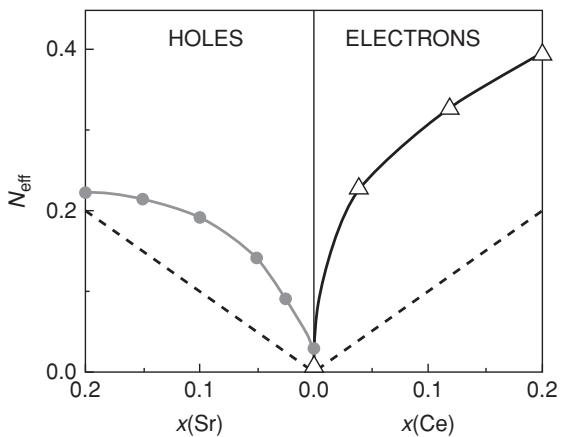
\includegraphics[width=0.55\textwidth]{figs/ch16/fig_16.11.jpg}
\caption*{图 16.11\quad 空穴掺杂（YBCO）与电子掺杂（$\mathrm{Nd}_{2-x}\mathrm{Ce}_x\mathrm{CuO}_4$，NCCO）铜氧化物的积分光电导，反映归一化载流子密度。虚线给出掺杂半导体的预期结果。在哈伯德模型内，超出名义掺杂量的电荷密度由动力学谱权重转移产生。翻印自 Cooper 等，Phys. Rev. B 41, 11605 (1990)。}\label{fig:auto:16.11}
\end{figure}
积分到光学能隙 $\Omega\approx 1.2\,\mathrm{eV}$ 为止。这是式 (9.143) 中 f 求和规则（f-sum rule）的一种形式。这里 $\sigma(\omega)$ 是光电导，$V_{\mathrm{cell}}$ 是每个化学式单胞的体积，$m$ 是自由电子质量，$e$ 是电子电荷。在没有掺杂、不形成金属态时，$N_{\mathrm{eff}}=0$。从图 16.11 可以明显看到，归一化载流子密度超过了把模型当作掺杂半导体所得的载流子密度（虚线）。在所有掺杂量下，对 $N_{\mathrm{eff}}=x$ 的偏离都是显著的。因此，任何只考虑名义掺杂量的模型都不足以描述铜氧化物中完整的低能电荷动力学。

\begin{figure}[H]\centering
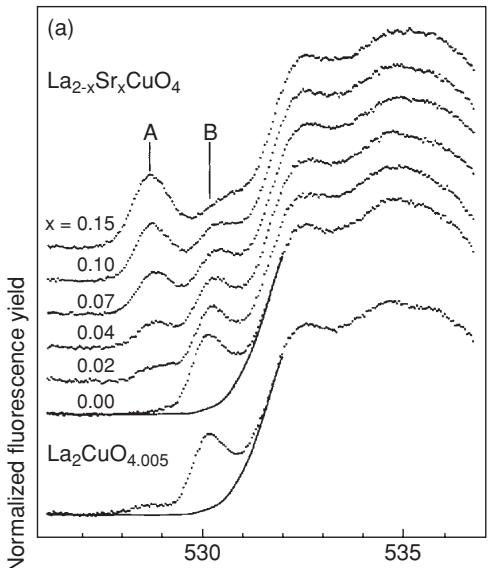
\includegraphics[width=0.5\textwidth]{figs/ch16/fig_16.12.jpg}

\vspace{0.5em}
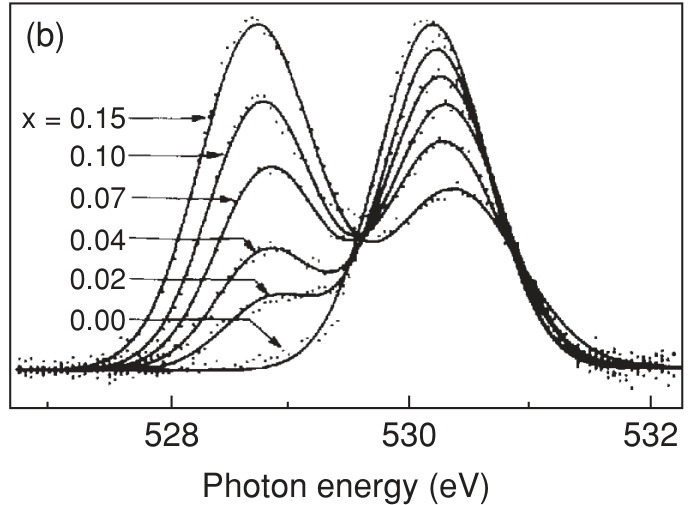
\includegraphics[width=0.6\textwidth]{figs/ch16/fig_16.12_b.jpg}
\caption*{图 16.12\quad $\mathrm{La}_{2-x}\mathrm{Sr}_x\mathrm{CuO}_{4+\delta}$ 氧 K 边的归一化荧光产额（[C1991]）。(a) 在未掺杂样品中，唯一的吸收出现在 530 eV 处，以 B 标记。掺杂后，B 处的强度转移到位于 528 eV 的 A 特征上。(b) 扣除背景后对 A、B 处吸收特征的高斯拟合。翻印自 Chen 等，Phys. Rev. Lett. 66, 104 (1991)。}\label{fig:auto:16.12}
\end{figure}
这一结果意义重大，因为它告诉我们：低能电荷自由度的数目超过裸掺杂量。因此，在强关联的语境下，最好考虑一个重正化的掺杂量 $x'\equiv x+\alpha$。本章的一个目的就是提出确定 $\alpha$ 的方法。本质上，在化学势所处的能带中，存在的并不只是裸电子。这看起来也许古怪，但事实上是真的，而且是强关联的普遍性以及谱的高、低能部分之间随之发生的混合的一部分。减去谱权重转移，得到的就是虚线（半导体）结果；然而，去掉谱权重转移同时也就去掉了强关联。最后一个值得一提的特征是 $N_{\mathrm{eff}}$ 在 $x=0$ 处的非零截距。这表明，即使在半填充，那些把莫特能隙以下的谱密度填补起来的激发仍有残余存在。这为我们理解图 16.11 中电荷计数超过虚线的起源提供了线索。

尽管光电导可用于提取有效载流子数，它终究是一个两粒子探针。因此，如果铜氧化物中载流子密度确实超过 $x$，那么从单粒子探针直接看到这一点会更有说服力。这确实可以做到。为此，我们分析图 16.12 所示的 $\mathrm{La}_{2-x}\mathrm{Sr}_x\mathrm{CuO}_4$（LSCO）的氧 $1s$ X 射线吸收实验（[C1991]）。在这类实验中，一个电子从芯态 $1s$ 被激发到一个未占据能级。实验可观测量是电子弛豫回到价态时荧光产额随能量的变化。图 16.12 的实验表明，$x=0$ 时所有可用的态都位于 530 eV 处。随掺杂增加，高能峰的强度减小，并转移到 528 eV 处的态。事实上，实验上（[C1991]）较低的峰按快于 $2x$ 的速率增长，而较高的峰按快于 $1-x$ 的速率减小，$x$ 为空穴数目。在 $\mathrm{La}_{2-x}\mathrm{Sr}_x\mathrm{CuO}_4$ 中，掺杂量 $x$ 可以毫不含糊地确定，因为每个 Sr 原子产生一个空穴。这两个峰之间的间隔就是母体绝缘材料的光学能隙。

实验中看到的谱权重的重新分布可以在哈伯德模型内得到解释。由于实验探测的是向可用的低能态的荧光产额，相应的理论量是每格点低能单粒子添加态的数目，
\begin{equation*}
L=\int_{\mu}^{\Lambda}N(\omega)\,\mathrm{d}\omega,\tag{16.117}
\end{equation*}
它定义为从化学势 $\mu$ 到截断能量尺度 $\Lambda$ 的单粒子态密度（$N(\omega)$）的积分，$\Lambda$ 划定了红外（IR）与紫外（UV）尺度的分界。费米液体中不存在上能带，$\Lambda$ 可以延伸到无穷大；而在半导体中，$\Lambda$ 只应延伸到价带顶，以计入添加空穴时可用的态。为标定这个量，我们把它与电子能够添加到掺杂剂所产生的空态上的方式数目相比较。记这个量为 $n_{\mathrm{h}}$。先考虑费米液体或无相互作用体系的情形。如图 16.2 所示，价带的总权重为 2，即每格点两个态。价带积分到化学势的权重决定填充。因此，决定 $L$ 的谱的未占据部分为 $L=2-n$。电子可以添加到空格点上的方式数目同样是 $n_{\mathrm{h}}=2-n$（见图 13.2）。于是，每电子每自旋的低能态数恒等于 1。这个结果赖以成立的关键事实是：价带总权重是一个与电子密度无关的常数。

现在考虑莫特绝缘体。在原子极限，我们已经确立（例如见式 (16.32)）：下能带的权重为 $1+x$。由于恰好有 $1-x$ 个被填充的态，$L=2x$ 在原子极限是严格的。也就是说，如图 16.4 所示，每个空穴留下一个可以被自旋向上或自旋向下电子占据的空格点。因此，基于哈伯德模型的原子极限，我们确实预期 LSCO 中 528 eV 处的荧光产额按正比于 $x$ 增长，同时在 530 eV——上哈伯德带所在的位置——有等效的减小。然而，从图 16.13 可以清楚看到，荧光产额的增长快于 $2x$。有限 $t/U$ 的哈伯德模型复现了这一结果。

\begin{figure}[H]\centering
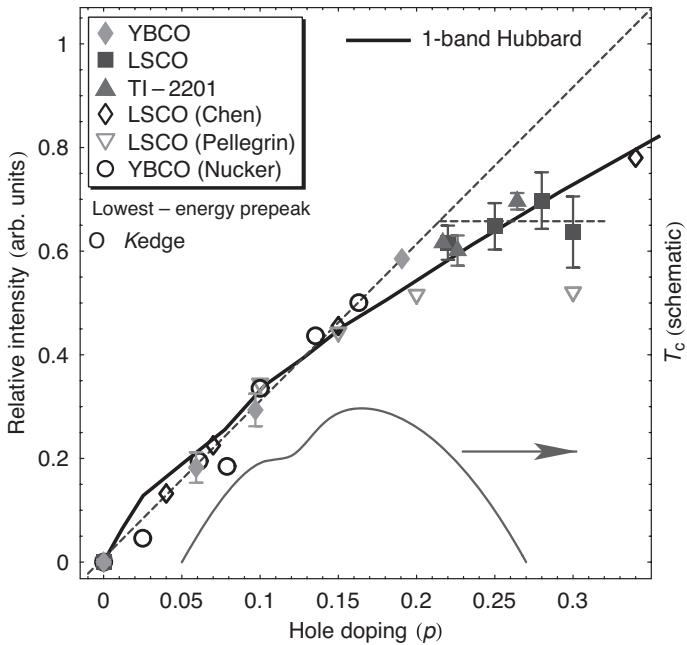
\includegraphics[width=0.62\textwidth]{figs/ch16/fig_16.13.jpg}
\caption*{图 16.13\quad 若干铜氧化物中最低能量氧 K 边前峰随掺杂变化的汇编。实直线是 A.~Liebsch（[L2010]）计算的哈伯德模型低能谱。由于实验数据的单位是任意的，用一个常数标度因子把 Liebsch 的数据点缩放后叠合到实验数据上。超导穹顶供参照。翻印自 Phillips 与 Jarrell，Phys. Rev. Lett. 105, 199701 (2010)。}\label{fig:auto:16.13}
\end{figure}

我们感兴趣的量 $L$ 可以从下能带的总权重
\begin{equation*}
m_{\mathrm{LHB}}=\frac{1}{N}\sum_{i}\big\langle\bigl\{c_{i\sigma;0},c_{i\sigma;0}^{\dagger}\bigr\}\big\rangle,\tag{16.118}
\end{equation*}
中简单地减去名义占据权重 $1-x$ 而得到。这里“名义”指的是由静态自由度确立的掺杂量，而不包括因动力学（$t/U$）效应进入的部分。这种混合意味着掺杂量本身被修改了，如图 16.11 所示。从投影到最低能量扇区的电子算符方程，即式 (16.110)，我们暂且把表达式简化为
\begin{equation*}
m_{\mathrm{LHB}}^{0}=\frac{1}{N}\sum_{i}\Big(\bigl\langle\bigl\{\tilde{\xi}_{i\sigma},\tilde{\xi}_{i\sigma}^{\dagger}\bigr\}\bigr\rangle+\Bigl\langle\frac{1}{U}\bigl(\bigl\{\tilde{\xi}_{i\sigma}^{\dagger},[\tilde{T}_{1},\tilde{\eta}_{i\sigma}]\bigr\}+\mathrm{h.c.}\bigr)\Bigr\rangle+\cdots\Big).\tag{16.119}
\end{equation*}
利用恒等式
\begin{equation*}
\tilde{\xi}_{i\sigma}\tilde{\eta}_{i\sigma}=\tilde{\xi}_{i\sigma}\tilde{\eta}_{i\sigma}^{\dagger}=0\tag{16.120}
\end{equation*}
以及基态性质 $\tilde{\eta}_{i\sigma}|G\rangle=0$，我们得到
\begin{equation*}
\big\langle\bigl\{\tilde{\xi}_{i\sigma}^{\dagger},[\tilde{T}_{1},\tilde{\eta}_{i\sigma}]\bigr\}\big\rangle=-\langle\tilde{\eta}_{i\sigma}\tilde{T}_{1}\tilde{\xi}_{i\sigma}^{\dagger}\rangle.\tag{16.121}
\end{equation*}
反复使用对易子
\begin{equation*}
\big[\tilde{n}_{i\bar{\sigma}},f_{j\sigma'}^{\dagger}\big]=\delta_{ij}\delta_{\bar{\sigma}\sigma'}f_{j\sigma'}^{\dagger},\tag{16.122}
\end{equation*}
可以把这个矩约化为两项之和：
\begin{align*}
-\langle\tilde{\eta}_{i\sigma}\tilde{T}_{1}\tilde{\xi}_{i\sigma}^{\dagger}\rangle
&=t\sum_{j,\delta,\sigma'}\big\langle f_{i\sigma}^{\dagger}\tilde{n}_{i\bar{\sigma}}\tilde{n}_{j\bar{\sigma}'}f_{j\sigma'}^{\dagger}f_{j+\delta\sigma'}(1-\tilde{n}_{j+\delta\bar{\sigma}'})(1-\tilde{n}_{i\bar{\sigma}})f_{i\sigma}^{\dagger}\big\rangle\\
&=t\sum_{j,\delta,\sigma'}\delta_{ij}\delta_{\bar{\sigma}\sigma'}\big\langle f_{i\sigma}^{\dagger}\tilde{n}_{j\bar{\sigma}'}f_{j\sigma'}^{\dagger}f_{j+\delta\sigma'}(1-\tilde{n}_{j+\delta\bar{\sigma}'})(1-\tilde{n}_{i\bar{\sigma}})f_{i\sigma}^{\dagger}\big\rangle\\
&\quad+t\sum_{j,\delta,\sigma'}\big\langle f_{i\sigma}^{\dagger}\tilde{n}_{j\bar{\sigma}'}f_{j\sigma'}^{\dagger}\tilde{n}_{i\bar{\sigma}}f_{j+\delta\sigma'}(1-\tilde{n}_{j+\delta\bar{\sigma}'})(1-\tilde{n}_{i\bar{\sigma}})f_{i\sigma}^{\dagger}\big\rangle\\
&=t\sum_{\delta}\big\langle f_{i\sigma}\tilde{n}_{i\sigma}f_{i\bar{\sigma}}^{\dagger}f_{i+\delta\bar{\sigma}}(1-\tilde{n}_{i+\delta\sigma})(1-\tilde{n}_{i\bar{\sigma}})f_{i\sigma}^{\dagger}\big\rangle\\
&\quad+t\sum_{j,\delta,\sigma'}\big\langle f_{i\sigma}^{\dagger}\tilde{n}_{j\bar{\sigma}'}f_{j\sigma'}^{\dagger}\tilde{n}_{i\bar{\sigma}}f_{j+\delta\sigma'}(1-\tilde{n}_{j+\delta\bar{\sigma}'})(1-\tilde{n}_{i\bar{\sigma}})f_{i\sigma}^{\dagger}\big\rangle,\tag{16.123}
\end{align*}
类似地使用式 (16.122) 中的对易子以及关系
\begin{equation*}
(1-\tilde{n}_{i\sigma})(1-\tilde{n}_{i\bar{\sigma}})f_{i\sigma}^{\dagger}=(1-\tilde{n}_{i\bar{\sigma}})(1-\tilde{n}_{i\sigma})f_{i\sigma}^{\dagger}=0\tag{16.124}
\end{equation*}
和
\begin{equation*}
\tilde{n}_{i\bar{\sigma}}(1-\tilde{n}_{j+\delta\bar{\sigma}'})(1-\tilde{n}_{i\bar{\sigma}})=(1-\tilde{n}_{j+\delta\bar{\sigma}'})\tilde{n}_{i\bar{\sigma}}(1-\tilde{n}_{i\bar{\sigma}})=0\tag{16.125}
\end{equation*}
可以证明，式 (16.123) 中的第二项
\begin{align*}
&\sum_{j,\delta,\sigma'}\big\langle f_{i\sigma}^{\dagger}\tilde{n}_{j\bar{\sigma}'}f_{j\sigma'}^{\dagger}\tilde{n}_{i\bar{\sigma}}f_{j+\delta\sigma'}(1-\tilde{n}_{j+\delta\bar{\sigma}'})(1-\tilde{n}_{i\bar{\sigma}})f_{i\sigma}^{\dagger}\big\rangle\\
&\quad=-t\sum_{j,\delta,\sigma'}\delta_{i,j+\delta}\delta_{\bar{\sigma}\sigma'}\big\langle f_{i\sigma}^{\dagger}\tilde{n}_{j\bar{\sigma}'}f_{j\sigma'}^{\dagger}f_{j+\delta\sigma'}(1-\tilde{n}_{j+\delta\bar{\sigma}'})(1-\tilde{n}_{i\bar{\sigma}})f_{i\sigma}^{\dagger}\big\rangle\\
&\qquad+t\sum_{j,\delta,\sigma'}\big\langle f_{i\sigma}^{\dagger}\tilde{n}_{j\bar{\sigma}'}f_{j\sigma'}^{\dagger}f_{j+\delta\sigma'}\tilde{n}_{i\bar{\sigma}}(1-\tilde{n}_{j+\delta\bar{\sigma}'})(1-\tilde{n}_{i\bar{\sigma}})f_{i\sigma}^{\dagger}\big\rangle\\
&\quad=-t\sum_{\delta}\big\langle f_{i\sigma}^{\dagger}\tilde{n}_{i-\delta\sigma}f_{i-\delta\bar{\sigma}}^{\dagger}f_{i\bar{\sigma}}(1-\tilde{n}_{i\sigma})(1-\tilde{n}_{i\bar{\sigma}})f_{i\sigma}^{\dagger}\big\rangle\\
&\qquad+t\sum_{j,\delta,\sigma'}\big\langle f_{i\sigma}^{\dagger}\tilde{n}_{j\bar{\sigma}'}f_{j\sigma'}^{\dagger}f_{j+\delta\sigma'}\tilde{n}_{i\bar{\sigma}}(1-\tilde{n}_{j+\delta\bar{\sigma}'})(1-\tilde{n}_{i\bar{\sigma}})f_{i\sigma}^{\dagger}\big\rangle=0\tag{16.126}
\end{align*}
恒为零。我们已接近完成。剩余项中还有几个因子可以用恒等式
\begin{align*}
f_{i\sigma}\tilde{n}_{i\sigma}&=f_{i\sigma},\\
f_{i\bar{\sigma}}^{\dagger}(1-\tilde{n}_{i\bar{\sigma}})&=f_{i\bar{\sigma}}^{\dagger}.\tag{16.127}
\end{align*}
加以简化。于是
\begin{align*}
-\langle\tilde{\eta}_{i\sigma}\tilde{T}_{1}\tilde{\xi}_{i\sigma}^{\dagger}\rangle
&=t\sum_{\delta}\big\langle f_{i\sigma}\tilde{n}_{i\sigma}f_{i\bar{\sigma}}^{\dagger}f_{i+\delta\bar{\sigma}}(1-\tilde{n}_{i+\delta\sigma})(1-\tilde{n}_{i\bar{\sigma}})f_{i\sigma}^{\dagger}\big\rangle\\
&=t\sum_{\delta}\big\langle f_{i\sigma}\tilde{n}_{i\sigma}f_{i\sigma}^{\dagger}f_{i\bar{\sigma}}^{\dagger}(1-\tilde{n}_{i\bar{\sigma}})f_{i+\delta\bar{\sigma}}(1-\tilde{n}_{i+\delta\sigma})\big\rangle\\
&=t\sum_{\delta}\big\langle f_{i\sigma}f_{i\sigma}^{\dagger}f_{i\bar{\sigma}}^{\dagger}f_{i+\delta\bar{\sigma}}(1-\tilde{n}_{i+\delta\sigma})\big\rangle\\
&=t\sum_{\delta}\Big\langle(1-\tilde{n}_{i\sigma})f_{i\bar{\sigma}}^{\dagger}f_{i+\delta\bar{\sigma}}(1-\tilde{n}_{i+\delta\sigma})\Big\rangle.\tag{16.128}
\end{align*}
由于平均是对一个不存在 $f_{i\sigma}$ 费米子双占据的基态作的，带密度因子 $\tilde{n}_{i\sigma}$ 的项全部消失，于是下能带的总权重
\begin{equation*}
m_{\mathrm{LHB}}=1+x+\frac{2t}{U}\frac{1}{N}\sum_{i\delta\sigma}\big\langle f_{i\bar{\sigma}}^{\dagger}f_{i+\delta\bar{\sigma}}\big\rangle+\cdots=1+x+\alpha(t/U,x)>1+x,\tag{16.129}
\end{equation*}
带有显式的 $t/U$ 修正，其第一项正比于下能带中因双占据的动力学产生而出现的空格点的动能。我们用 $\alpha$ 表示所有 $t/U$ 修正，它是谱权重动力学转移的量度。这个公式的一个版本最初由 Harris 与 Lange（[HL1967]）于 1967 年导出，并在文献 [E1994] 中用正确的算符重新导出。值得注意的是，出现在这个表达式中的算符是变换后的费米子，而不是裸费米子。当然，可以只用裸费米子表示下能带的谱权重，但表达式相当繁琐（[E1994]）。同样值得注意的是，无论微扰论的阶数如何，$\alpha$ 都严格为正（[HL1967; E1994; MES1993]）。道理很简单：下能带中的动力学只能以产生双占据格点为代价。这必然使上能带的强度减小（见图 16.14），因为现在产生双占据的方式变少了。为保持谱权重守恒，下能带的强度必须增加同等的量。本质上，动力学谱权重转移之所以存在，是因为算符 $\xi_{i\sigma}$ 与 $\eta_{i\sigma}$ 在任何能量尺度上都不能独立传播。若把下能带谱的占据部分赋以守恒电荷 $1-x$ 的权重，则下能带谱的未占据部分携带权重 $2x+\alpha>2x$。然而，没有必要固守对谱的这种划分，因为一旦一个能带的权重超过该能带中电子态的总数，即 $1+x+\alpha>1+x$，电子究竟在做什么就无关紧要了。我们从图 16.11 知道，有效掺杂量超过 $x$。图 16.14(b) 中对谱权重的划分（[CHP2010]）反映了载流子的动力学产生。采用这种划分，LHB 中每自旋的谱未占据部分恰好就是有效掺杂量 $x'$。也就是说，对谱的这种划分恢复了原子极限下的半刚性能带图像，如图 16.4 那样。图 16.13 把 $L$ 的实验值与哈伯德模型上最先进的计算（实线）作了比较。解读实验值时需要提醒一句。由于强度是用任意单位表示的，$y$ 轴并不真正对应能带未占据部分的实际谱密度。注意虚线的斜率为 3。因此，不应把这条直虚线理解为氧 K 边谱按 $2x$ 增长的量度。为了在哈伯德模型的结果与实验之间进行比较，哈伯德数据经过了适当的标度。引人注目的是，在所研究的掺杂范围内，实线与实验值在定量上符合得相当好。在空穴掺杂量 $p\approx 0.18$ 附近，数据与虚线（它从原点出发）有明显偏离。哈伯德模型同样复现了这一偏离，它标志着超过某个临界掺杂值之后，动力学修正急剧减小。原因很简单：动力学修正必须在 $x=1$ 处消失，因此它不可能单调增加。

\begin{figure}[H]\centering
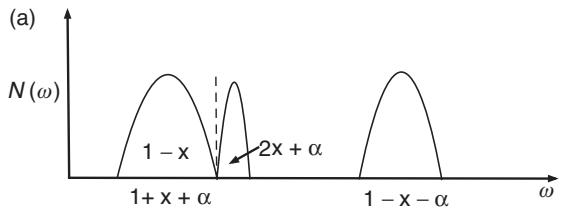
\includegraphics[width=0.62\textwidth]{figs/ch16/fig_16.14_a.jpg}

\vspace{0.5em}
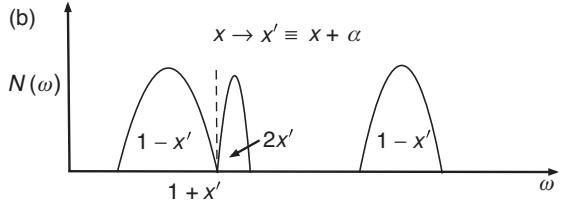
\includegraphics[width=0.62\textwidth]{figs/ch16/fig_16.14_b.jpg}
\caption*{图 16.14\quad 哈伯德模型中单粒子态密度随空穴掺杂量 $x$ 的变化。$\alpha$ 表示式 (16.129) 所刻画的谱权重的动力学即 $t/U$ 修正。(a) 下能带谱权重的传统划分，其中下能带被占据的部分就是守恒电荷。(b) 计及图 16.11 中所见掺杂量重正化的谱权重划分。}\label{fig:auto:16.14}
\end{figure}

$d=1$ 的哈伯德模型为计算 $\alpha$ 提供了一个基准。在这种情形下，$\alpha$ 可以用贝特拟设（Bethe ansatz）（[LW1968]）方法结合动力学矩阵重正化群（[K2010]）来计算进入谱函数的动力学关联函数，从而基本上精确地确定。图 16.15 给出了下哈伯德带中谱密度在化学势以下（方块）和以上的积分权重的结果。图 16.15 中的星号代表谱的占据部分，$1-x$。每自旋其余的谱权重（圆圈，$U=4t$；方块，$U=8t$）给出 $L$（按照图 16.14(a) 计算）的量度。显然，两者都超过虚线，正如式 (16.129) 的微扰展开所预期，并与图 16.13 所示的二维计算一致。一般地，对任何有限维晶格，动力学谱权重转移都是不可避免的。

\begin{figure}[H]\centering
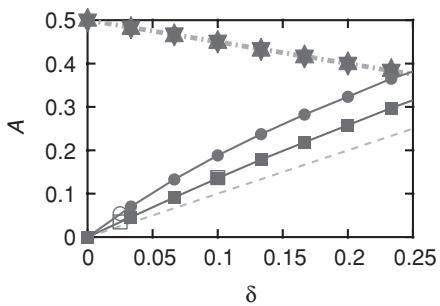
\includegraphics[width=0.5\textwidth]{figs/ch16/fig_16.15.jpg}
\caption*{图 16.15\quad $d=1$ 哈伯德模型中下能带每自旋的积分谱权重。星号代表下能带的占据部分。实心方块与圆圈分别对应 $U=8t$ 和 $U=4t$ 时的粒子添加部分（恰在化学势之上）。虚线的斜率为 1。翻印自 Kohno，Phys. Rev. Lett. 105, 106402 (2010)。}\label{fig:auto:16.15}
\end{figure}

动力学谱权重转移之所以重要，是因为它产生了一种全新的定性效应。它是“多”则全然不同（``more'' being totally different）的一个例子（[A1972]）。费米液体中，一个能带的强度等于该能带所能容纳的电子数。而在存在动力学谱权重转移时，下能带和能带未占据部分的强度都超过这些态在低能下所能容纳的电子数，与费米液体形成鲜明对照。能装进下能带的电子数只由格点数目决定，而不依赖于诸如 $t$ 和 $U$ 这样的体系参数，因此它固定在 $1+x$。同样，下能带谱的未占据部分只能以 $2x$ 种方式被电子占据。然而，至少有 $2x+\alpha$ 个态可供粒子添加。结果，对下能带物理的任何描述都无法仅凭数电子来穷尽。本质上，如果一个能带的总谱权重超过电子计数——此处即 $1+x+\alpha>1+x$——那么电子究竟在做什么就无关紧要。这凸显了强耦合的关键要素：传播自由度与原始紫外完备理论中的基本构件毫无相似之处。例如考虑 $L$。$L$ 量度的是向 下能带添加一个粒子的总谱密度。若它按每自旋超过 $x$，则添加一个粒子的方式总数超过向下能带添加一个\emph{电子}的方式数。因此，$L/2>x$ 意味着下能带中有些粒子添加态对添加一个电子是有能隙的。也就是说，下能带中有些态与添加一个电子正交。产生这种正交性的态是与上能带混合的态。因此，正是上能带的单纯存在在下能带中产生了这段有能隙的谱。既然上能带完全源于强关联，混入下能带的这些额外的态在弱相互作用体系中没有对应物，费米液体理论便告失效。由此，动力学谱权重转移为下能带中有效费米液体描述的失效提供了一个具体机制。虽然安德森（[A1997]）早先已假定上哈伯德带会在低能下导致对电子添加的正交性，但他并未明确把动力学谱权重转移指认为这种正交性的具体机制。事实上，他近期的工作（[A2006]）专注于严格从 $U=\infty$ 极限——动力学修正在此消失——提取这种正交性。

\begin{figure}[H]\centering
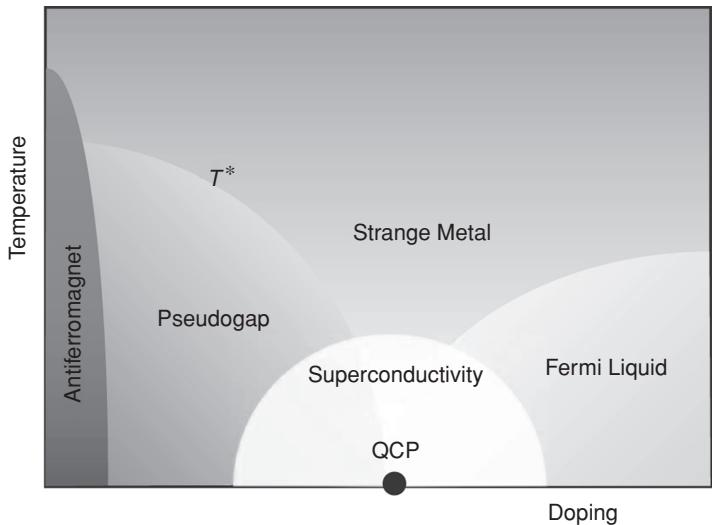
\includegraphics[width=0.7\textwidth]{figs/ch16/fig_16.16.jpg}
\caption*{图 16.16\quad 掺入铜氧面的空穴浓度的示意相图。赝能隙与奇异金属分别以态密度的亏耗和 $T$ 线性电阻率为特征。赝能隙终止于一个零温临界点，即量子临界点（QCP）。右侧是弱耦合描述成立的费米液体区。}\label{fig:auto:16.16}
\end{figure}

对电子添加的正交性是铜氧化物正常态的核心问题。图 16.16 给出了铜氧化物的示意相图，其中突出标出了掺杂莫特绝缘体后出现的关键角色。赝能隙与奇异金属是正常态中我们关心的两个相。在赝能隙区，存在能隙但没有超导。与费米液体不同，奇异金属表现出 $T$ 线性电阻率。的确，正如相图所提示的，奇异金属与赝能隙紧密相连。实验上，$T^{*}$ 线由输运测量确定为 $T$ 线性电阻率出现的最低温度（[KLR2001; AKS2004]）。由于超导态具有 $d_{x^{2}-y^{2}}$ 对称性（[H1995]），布里渊区对角线代表节点方向。图 16.17 绘出的是对铜氧化物中沿布里渊区对角线的电子格林传播子的极点
\begin{equation*}
G(\omega,\mathbf{q})=\frac{Z}{\omega-\epsilon_{\mathrm{F}}}\tag{16.130}
\end{equation*}
强度的高精度测量。关于式 (16.130) 的解读需要说明几句。即使电子传播子带有如式 (16.58) 那样的自能，像式 (16.130) 这样的表达式仍然成立。只需围绕费米能展开自能，
\begin{equation*}
\Sigma(\omega,\mathbf{k})=\Sigma_{0}+(\omega-\epsilon_{\mathrm{F}})\frac{\partial\Sigma^{\mathrm{R}}(\omega,\mathbf{k})}{\partial\omega}\Big|_{\omega=\epsilon_{\mathrm{F}}}+\cdots,\tag{16.131}
\end{equation*}

\begin{figure}[H]\centering
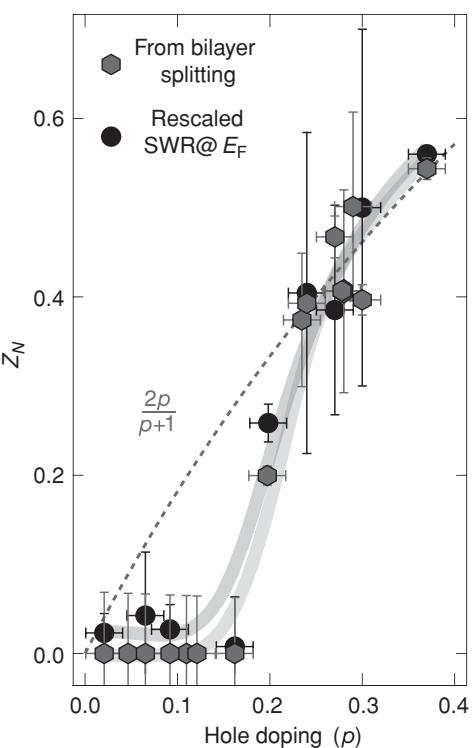
\includegraphics[width=0.45\textwidth]{figs/ch16/fig_16.17.jpg}
\caption*{图 16.17\quad YBCO 中由角分辨光电子能谱测得的准粒子权重。准粒子权重的消失表明铜氧化物的正常态是非费米液体。翻印自 Fournier 等，Nat. Phys. 6, 905 (2010)。}\label{fig:auto:16.17}
\end{figure}
只保留一阶导数项，我们把准粒子权重表示为
\begin{equation*}
Z=(1-\partial\Sigma^{\mathrm{R}}/\partial\omega)^{-1}.\tag{16.132}
\end{equation*}
费米液体中，每个掺杂剂都在化学势上方产生一个准粒子激发，因此准粒子权重预期按 $x$ 标度。铜氧化物中情形并非如此。令人注目的是，准粒子权重（[F2010]）在掺杂量 0.15 附近消失，表明超导电性由之涌现的底层状态是一个非费米液体，其中电子并不是传播自由度。传播模式究竟是什么，正是铜氧化物的核心问题。图 16.17 用来比较准粒子权重的理论（[A2004]）给出 $Z\propto 2x/(1+x)$。这个表达式只应在 $x=0$ 处消失。该公式的来历不过是把准粒子权重的费米液体形式应用于静态部分，即严格从下能带谱权重的态计数得出的那部分。按照费米液体理论，准粒子权重应按谱的未占据部分、并以能带的总强度加权来标度。既然有 $2x$ 个粒子添加态，而能带的总权重为 $1+x$，结果 $Z=2x/(1+x)$ 是自然的。然而，数据（见图 16.17）表明该公式失效。

如上所述，动力学谱权重转移为费米液体理论的失效、从而为 $Z$ 的消失提供了一个自然机制。归根到底，如果动力学谱权重转移是费米液体理论失效的机制，那么这种物理在超导态中应当仍然存在，因为它对有序化并不敏感。事实确实如此。为引导这里的讨论，我们关注 f 求和规则
\begin{equation*}
A=\frac{\pi n_{e}e^{2}}{m}=\int_{0}^{\infty}\sigma(\omega)\,\mathrm{d}\omega.\tag{16.133}
\end{equation*}
为理解高 $T_{\mathrm{c}}$ 超导体中的谱变化，把 $A$ 分解为低能分量
\begin{equation*}
A_{\mathrm{l}}=\int_{0^{+}}^{\Omega}\sigma(\omega)\,\mathrm{d}\omega,\tag{16.134}
\end{equation*}
和高能部分
\begin{equation*}
A_{\mathrm{h}}=\int_{\Omega}^{\infty}\sigma(\omega)\,\mathrm{d}\omega.\tag{16.135}
\end{equation*}
是有帮助的。截断 $\Omega$ 的选取使得 $A_{\mathrm{h}}$ 严格包含与带间跃迁相联系的谱权重。通常取 $\Omega/(2\pi c)=10\,000\,\mathrm{cm}^{-1}$ 便足以界定 $\sigma(\omega)$ 的极小值，该极小值标志带内跃迁与带间跃迁的分界，本质上就是下、上哈伯德带之间的截断。回忆式 (9.136)，电导率有如下形式的虚部
\begin{equation*}
\mathrm{Im}\,\sigma(\omega)=\frac{n_{e}e^{2}/m}{\omega}.\tag{16.136}
\end{equation*}
只有在超导体中，这一贡献才不为零。由克拉默斯—克勒尼希（Kramers--Kronig）关系
\begin{equation*}
\mathrm{Im}\,\sigma(\omega)=\frac{1}{\pi}\,\mathrm{P}\int_{-\infty}^{\infty}\frac{\mathrm{d}\omega'\,\mathrm{Re}\,\sigma(\omega')}{\omega'-\omega},\tag{16.137}
\end{equation*}
与式 (16.136) 相容的电导率实部为 $\mathrm{Re}\,\sigma(\omega)=A\delta(\omega)$。在超导体中，$\hbar\omega<2\Delta$（$\Delta$ 为超导能隙）范围内被移走的谱权重转移到零频率处的 $\delta$ 函数上。$\delta$ 函数中的权重必定等于凝聚到超导态时被移走的谱权重。这一效应由 Ferrell--Glover--Tinkham（[T2004]）求和规则描述：
\begin{equation*}
D=A_{\mathrm{l}}^{\mathrm{n}}-A_{\mathrm{l}}^{\mathrm{s}}+A_{\mathrm{h}}^{\mathrm{n}}-A_{\mathrm{h}}^{\mathrm{s}},\tag{16.138}
\end{equation*}
其中上标 n 与 s 分别指正常态与超导态。BCS 超导体的特征是高、低能量尺度之间有清晰的分界，$D$ 中没有来自 $A_{\mathrm{h}}$ 的贡献。通常，只需积分到不超过 $10\Delta$ 便能恢复 $D$。然而，在高 $T_{\mathrm{c}}$ 超导体中，椭偏实验（[RG2001]）观察到介电函数在转变到超导态时的变化延伸到 $100\Delta$，这对铜氧化物而言暗示了另一种情形。

\begin{figure}[H]\centering
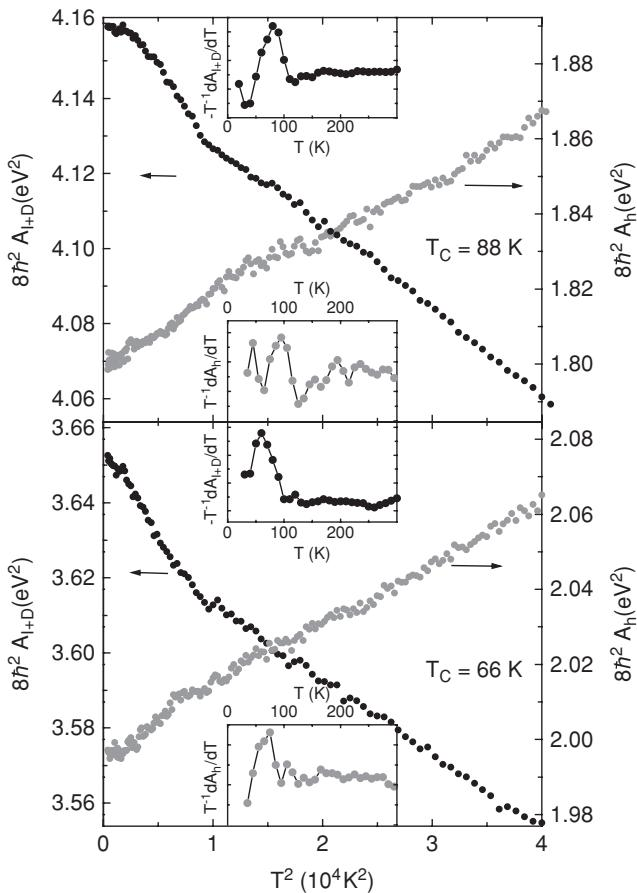
\includegraphics[width=0.48\textwidth]{figs/ch16/fig_16.18.jpg}
\caption*{图 16.18\quad 最佳掺杂（上）与欠掺杂（下）的 $\mathrm{Bi}_2\mathrm{Sr}_2\mathrm{CaCu}_2\mathrm{O}_{8-\delta}$ 的低频谱权重 $A_{\mathrm{l}+D}(T)$ 与高频谱权重 $A_{\mathrm{h}}(T)$ 随温度的变化。插图给出这两个量的导数乘以 $T^{-1}$。翻印自 Molegraaf 等，Science 295, 5563 (2002)。}\label{fig:auto:16.18}
\end{figure}

对 BSCCO（译注：原文为 BSCO）（[M2002]），无论最佳掺杂还是欠掺杂样品，当温度降到 $T_{\mathrm{c}}$ 以下时，$A_{\mathrm{h}}$ 表现出加速的减小，同时 $A_{\mathrm{l}}$ 补偿性地增加，如图 16.18 所示。这表明，正是高能区谱权重的损失驱动了超导态。这些数据还与其他光学测量一致——后者表明，把光电导积分到 2 eV 便能恢复超导态中 $\delta$ 函数的全部权重（[SL2003]）；也与数值计算一致——后者表明，哈伯德模型中随频率变化的配对相互作用包含一个完全来自上哈伯德带的非推迟部分（[MPS2008]）。这种从可见光到红外波段的“变色”意味着，铜氧化物中的超导电性与金属中的存在本质差别。也就是说，在铜氧化物中，超导电性并非只关乎费米面上的低能物理。正确的理论应当精确解释，高能处（距化学势 2 eV）的谱权重损失如何导致超流密度的增长。

\section{尾声：$1=2-1$}

正如我们所见，铜氧化物体现了固体物理学三大支柱的失效：(1) 金属的能带论，(2) 费米液体理论，(3) 超导电性的 BCS 理论。这一概念三联体的核心是刚性带概念的缺席。如本章开头所述，UHB 与 LHB 并非传统意义上的能带。尽管如此，我们可以遵循上文概述的微扰流程，依据在原子极限中获得的直觉对谱进行划分。式 (16.129) 意味着，下能带的总强度超过 $1+x$，即下能带中电子态的总数。动力学修正 $\alpha$ 在实验上可以直接观测：既可以在 X 射线 K 边实验（[C1991]）中，也可以在光学测量（[C1990]）中，这些测量表明有效掺杂量超过裸空穴计数 $x$。一个能带的强度怎么可能超过该能带中电子态的数目？能带中显然必定还有别的东西，而且它必定携带电荷 $e$，因为强度所计数的正是电荷为 $e$ 的激发的数目。这些额外的电荷 $e$ 激发是什么？我们有两种选择：要么把电子的自旋与电荷拆开，要么选择复合激发。把自旋与电荷拆开并不能解决额外强度的问题，因为这不可能给出大于 $1+x$ 的强度。唯一的选择是复合激发。本节标题中的那个方程给出了答案：$1=2-1$。一个电荷为 $2e$ 的实体与电荷为 $-e$ 的空穴相束缚，正合所需。结果是一个电荷为 $e$ 的复合激发。可以想象更复杂的方案，但 $1=2-1$ 是最简单的。而且，这在物理上是合理的。动力学谱权重转移所涉及的，恰恰就是莫特（[M1949]）以及其他人（[KHF1982; K1964; C1979]）论证过必须束缚在一起以传递莫特能隙的那类激发（见图 16.7）。有限掺杂时，这类激发依然存在。它们代表双占据格点与空格点上的空穴之间的束缚态，从而为 $1=2-1$ 提供了一条物理途径。本质上，低能下的双占据代表一种集体激发，它源于下、上能带刚性的缺失。这种激发可以在一个场论中具体实现（[LPC2007; P2010]）：对上能带引入一个约束，使得约束保持时上能带是刚性的；一旦约束放宽，一个电荷为 $2e$ 的玻色场就会作为低能集体激发出现，正如电子气问题中，一旦放宽对扩展希尔伯特空间的约束，等离激元便应运而生。事实上，严格积掉上哈伯德带所用的技巧（[LPC2007; P2010]）（超出了本书的范围）与第 9 章在等离激元的语境中引入的集体场论方法完全相同。一个电荷为 $2e$ 的集体场（显然是玻色性的，且不同于诸如库珀对之类的任何东西。库珀对由基本激发构成；而电荷 $2e$ 玻色子源于动力学，因而并非如此）在低能出现，并与空穴相束缚，这正是强耦合物理的典型表现。具体地说，新的激发（通常是复合物）作为低能的传播自由度出现，它们在紫外完备理论中没有对应物。这类激发也解决了图 16.17 中的正交性问题。由于它们拥有内部自由度，它们与裸电子正交，从而为图 16.17 中 $Z\to 0$ 的问题提供了一种解决之道。于是，简单的方程 $1=2-1$ 包含了动力学谱权重转移的精髓。图 16.18 的实验表明，负责动力学谱权重转移的这类激发，在铜氧化物的超导问题中扮演着关键却未知的角色。

\section*{习题}
\addcontentsline{toc}{section}{习题}

\textbf{习题 16.1}\quad 计及最近邻相互作用的哈伯德模型具有形式
\begin{equation*}
H_{\mathrm{Hubb}}=-t\sum_{i,j,\sigma}\big(\eta_{i\sigma}^{\dagger}\eta_{j\sigma}+\xi_{i\sigma}^{\dagger}\xi_{j\sigma}+\eta_{i\sigma}^{\dagger}\xi_{j\sigma}\big)+\frac{U}{2}\sum_{i,\sigma}\eta_{i\sigma}^{\dagger}\eta_{i,\sigma}+V\sum_{i,j}n_{i}n_{j},\tag{16.139}
\end{equation*}
其中 $n_{i}=n_{i\uparrow}+n_{i\downarrow}$。证明：使该模型在式 (16.39) 之下保持不变的化学势取值为 $\mu=(U+2V)/2$。

\textbf{习题 16.2}\quad 显式证明系数为
\begin{align*}
\alpha_{n+1}&=(U-\mu)\alpha_{n}+U(-\mu)^{n},\\
\beta_{n}&=(-\mu)^{n},\tag{16.140}
\end{align*}
所用的递推关系是
\begin{equation*}
Q_{i\sigma}^{(n+1)}=\big[Q_{i\sigma}^{(n)},H_{U}\big].\tag{16.141}
\end{equation*}

\textbf{习题 16.3}\quad 导出半填充哈伯德二聚体的所有本征态和本征值。所谓半填充，我指的是两个电子占据两个格点，一个自旋向上，另一个自旋向下。对基态，你应当得到式 (16.80)。

\textbf{习题 16.4}\quad 考虑一个算符 $O$。一般地
\begin{equation*}
O=\sum_{n\in\mathbb{Z}}O_{nU}.\tag{16.142}
\end{equation*}
你的任务是用变换后的算符 $\tilde{O}$ 导出 $O_{nU}$ 的显式表达式。由一般表达式
\begin{equation*}
O=\mathrm{e}^{S}\tilde{O}\mathrm{e}^{-S}\tag{16.143}
\end{equation*}
证明
\begin{align*}
O_{nU}&=\tilde{O}_{nU}+\frac{1}{U}\big[\tilde{T}_{1},\tilde{O}_{(n-1)U}\big]-\frac{1}{U}\big[\tilde{T}_{-1},\tilde{O}_{(n+1)U}\big]\\
&\quad+\frac{1}{U^{2}}\Big(\big[\big[\tilde{T}_{1},\tilde{T}_{0}\big],\tilde{O}_{(n-1)U}\big]+\big[\big[\tilde{T}_{-1},\tilde{T}_{0}\big],\tilde{O}_{(n+1)U}\big]\\
&\quad+\frac{1}{2}\big[\tilde{T}_{1},\big[\tilde{T}_{1},\tilde{O}_{(n-2)U}\big]\big]+\frac{1}{2}\big[\tilde{T}_{-1},\big[\tilde{T}_{-1},\tilde{O}_{(n+2)U}\big]\big]\\
&\quad-\frac{1}{2}\big[\tilde{T}_{1},\big[\tilde{T}_{-1},\tilde{O}_{nU}\big]\big]-\frac{1}{2}\big[\tilde{T}_{-1},\big[\tilde{T}_{1},\tilde{O}_{nU}\big]\big]\Big).\tag{16.144}
\end{align*}

\section*{参考文献}
\addcontentsline{toc}{section}{参考文献}

\begin{itemize}[leftmargin=2em,itemsep=0pt,parsep=0pt,label={}]
\item {[AZ1988]} I.~Affleck, Z.~Zou, T.~Hsu, and P.~W. Anderson, \emph{Phys. Rev. B} \textbf{38}, 745 (1988).
\item {[A1972]} This is a rephrasing of the essay title ``More is Different'' by P.~W. Anderson, \emph{Science} \textbf{177}, 393 (1972).
\item {[A1987]} P.~W. Anderson, \emph{Science} \textbf{235}, 1196 (1987).
\item {[A1997]} P.~W. Anderson, \emph{The Theory of Superconductivity in the High-$T_{c}$ Cuprates} (Princeton Series in Physics, Princeton University Press, 1997).
\item {[A2006]} P.~W. Anderson, \emph{Nat. Phys.} \textbf{2}, 626 (2006).
\item {[A2004]} P.~W. Anderson, P.~A. Lee, M.~Randeria, T.~M. Rice, N.~Trivedi, and F.~C. Zhang, \emph{J. Phys.: Cond. Matt.} \textbf{16}, R755 (2004).
\item {[AKS2004]} Y.~Ando, S.~Komiya, K.~Segawa, S.~Ono, and Y.~Kurita, \emph{Phys. Rev. Lett.} \textbf{93}, 267001 (2004).
\item {[C1979]} C.~Castellani, C.~Di Castro, D.~Feinberg, and J.~Ranninger, \emph{Phys. Rev. Lett.} \textbf{43}, 1957 (1979).
\item {[CHP2010]} S.~Chakraborty, S.~Hong, and P.~Phillips, \emph{Phys. Rev. B} \textbf{81}, 235135 (2010).
\item {[C1991]} C.~T. Chen, F.~Sette, Y.~Ma, \emph{et al.}, \emph{Phys. Rev. Lett.} \textbf{66}, 104 (1991).
\item {[C2004]} A.~L. Chernyshev, D.~Galanakis, P.~Phillips, A.~V. Rozhkov, and A.-M.~S. Tremblay, \emph{Phys. Rev. B} \textbf{70}, 235111 (2004).
\item {[C1990]} S.~L. Cooper, G.~A. Thomas, J.~Ornstein, \emph{et al.}, \emph{Phys. Rev. B} \textbf{41}, 11605 (1990).
\item {[C1993]} S.~L. Cooper, D.~Reznik, A.~Kotz, \emph{et al.}, \emph{Phys. Rev. B} \textbf{47}, 8233 (1993).
\item {[DFM1988]} E.~Dagotto, E.~Fradkin, and A.~Moreo, \emph{Phys. Rev. B} \textbf{38}, 2926 (1988).
\item {[D2003]} I.~Dzyaloshinskii, \emph{Phys. Rev. B} \textbf{68}, 085113 (2003).
\item {[E1994]} H.~Eskes, A.~M. Ole\'{s}, M.~B.~J. Meinders, and W.~Stephan, \emph{Phys. Rev. B} \textbf{50}, 17980 (1994).
\item {[F2010]} D.~Fournier, G.~Levy, Y.~Pennec, \emph{et al.}, \emph{Nat. Phys.} \textbf{6}, 905 (2010).
\item {[GKKR1996]} A.~Georges, G.~Kotliar, W.~Krauth, and M.~J. Rozenberg, \emph{Rev. Mod. Phys.} \textbf{68}, 13 (1996).
\item {[G1971]} J.~B. Goodenough, \emph{J. Solid State Chem.} \textbf{3}, 490 (1971).
\item {[H1991]} F.~D.~M. Haldane, \emph{Phys. Rev. Lett.} \textbf{67}, 937 (1991).
\item {[H1995]} D.~J. van Harlingen, \emph{Rev. Mod. Phys.} \textbf{67}, 515 (1995).
\item {[HL1967]} A.~B. Harris and R.~V. Lange, \emph{Phys. Rev.} \textbf{157}, 295 (1967).
\item {[H1974]} G.~'t Hooft, \emph{N. Phys. B} \textbf{75}, 461 (1974).
\item {[H1963]} J.~Hubbard, \emph{Proc. Roy. Soc. London, Ser. A}, \textbf{276}, 238 (1963).
\item {[J1992]} M.~Jarrell, \emph{Phys. Rev. Lett.} \textbf{69}, 168 (1992).
\item {[KHF1982]} T.~A. Kaplan, P.~Horsch, and P.~Fulde, \emph{Phys. Rev. Lett.} \textbf{49}, 889 (1982).
\item {[K1964]} W.~Kohn, \emph{Phys. Rev.} \textbf{133}, A171 (1964).
\item {[K2010]} M.~Kohno, \emph{Phys. Rev. Lett.} \textbf{105}, 106402 (2010).
\item {[KLR2001]} Z.~Konstantinovic, Z.~Z. Li, and H.~Raffy, \emph{Physica C} \textbf{351}, 1653 (2001).
\item {[L2005]} Y.~S. Lee, K.~Segawa, Z.~Q. Li, \emph{et al.}, \emph{Phys. Rev. B} \textbf{72}, 054529 (2005).
\item {[LPC2007]} R.~G. Leigh, P.~Phillips, and T.-P. Choy, \emph{Phys. Rev. Lett.} \textbf{99}, 046404 (2007).
\item {[LW1968]} E.~H. Lieb and F.~Y. Wu, \emph{Phys. Rev. Lett.} \textbf{20}, 1445 (1968).
\item {[L2010]} A.~Liebsch, \emph{Phys. Rev. B} \textbf{81}, 235133 (2010).
\item {[MPS2008]} T.~A. Maier, D.~Poilblanc, and D.~J. Scalapino, \emph{Phys. Rev. Lett.} \textbf{100}, 237001 (2008).
\item {[MES1993]} M.~B.~J. Meinders, H.~Eskes, and G.~A. Sawatzky, \emph{Phys. Rev. B} \textbf{48}, 3916 (1993).
\item {[M2002]} H.~J.~A. Molegraaf, C.~Presura, D.~van der Marel, P.~H. Kes, and M.~Li, \emph{Science} \textbf{295}, 2239 (2002).
\item {[M1949]} N.~F. Mott, \emph{Proc. Phys. Soc. A} \textbf{62}, 416 (1949).
\item {[P2010]} P.~Phillips, \emph{Rev. Mod. Phys.} \textbf{82}, 1719 (2010).
\item {[Q2008]} M.~M. Qazilbash, A.~A. Schafgans, K.~S. Burch, \emph{et al.}, \emph{Phys. Rev. B} \textbf{77}, 115121 (2008).
\item {[RLP1994]} T.~M. Rice, H.~Launois, and J.~P. Pouget, \emph{Phys. Rev. Lett.} \textbf{73}, 3042 (1994).
\item {[R2007]} A.~Rosch, \emph{Eur. Phys. J. B} \textbf{59}, 495 (2007).
\item {[RG2001]} M.~R\"{u}bhausen, A.~Gozar, M.~V. Klein, P.~Guptasarma, and D.~G. Hinks, \emph{Phys. Rev. B} \textbf{63}, 224514 (2001).
\item {[SL2003]} A.~F. Santander-Syro, R.~P.~S.~M. Lobo, N.~Bontemps, Z.~Konstantinovic, Z.~Z. Li, and H.~Raffy, \emph{Eur. Phys. Lett.} \textbf{62}, 568 (2003).
\item {[SPC2007]} T.~D. Stanescu, P.~Phillips, and T.-P. Choy, \emph{Phys. Rev. B} \textbf{75}, 104503 (2007).
\item {[S2010]} I thank M.~Sobol for suggesting presenting the Mott problem starting from this model.
\item {[T2004]} M.~Tinkham, \emph{Introduction to Superconductivity} (Dover, 2004), 2nd edition.
\item {[ZR1988]} F.~C. Zhang and T.~M. Rice, \emph{Phys. Rev. B} \textbf{37}, 3759 (1988).
\item {[ZM1975]} A.~Zylbersztejn and N.~F. Mott, \emph{Phys. Rev. B} \textbf{11}, 4383 (1975).
\end{itemize}
